%%%%%%%%%%%%%%%%%%%%%%%%%%%%%%%%%%%%%%%%%%%%%%%%%%%%%%%%%%%%
%%% LIVECOMS ARTICLE TEMPLATE FOR BEST PRACTICES GUIDE
%%% ADAPTED FROM ELIFE ARTICLE TEMPLATE (8/10/2017)
%%%%%%%%%%%%%%%%%%%%%%%%%%%%%%%%%%%%%%%%%%%%%%%%%%%%%%%%%%%%
%%% PREAMBLE
\documentclass[9pt,tutorial]{livecoms}
% Use the 'onehalfspacing' option for 1.5 line spacing
% Use the 'doublespacing' option for 2.0 line spacing
% Use the 'lineno' option for adding line numbers.
% Use the "ASAPversion' option following article acceptance to add the DOI and relevant dates to the document footer.
% Use the 'pubversion' option for adding the citation and publication information to the document footer, when the LiveCoMS issue is finalized.
% The 'bestpractices' option for indicates that this is a best practices guide.
% Omit the bestpractices option to remove the marking as a LiveCoMS paper.
% Please note that these options may affect formatting.

\usepackage{lipsum} % Required to insert dummy text
\usepackage[version=4]{mhchem}
\usepackage{siunitx}
\DeclareSIUnit\Molar{M}
\usepackage[italic]{mathastext}
\usepackage{hyperref}
\graphicspath{{figures/}}

%%%%%%%%%%%%%%%%%%%%%%%%%%%%%%%%%%%%%%%%%%%%%%%%%%%%%%%%%%%%
%%% IMPORTANT USER CONFIGURATION
%%%%%%%%%%%%%%%%%%%%%%%%%%%%%%%%%%%%%%%%%%%%%%%%%%%%%%%%%%%%

\newcommand{\versionnumber}{0.1}  % you should update the minor version number in preprints and major version number of submissions.
\newcommand{\githubrepository}{\url{https://github.com/delphi001/delphi_tutorial_livecoms}}  %this should be the main github repository for this article

%%%%%%%%%%%%%%%%%%%%%%%%%%%%%%%%%%%%%%%%%%%%%%%%%%%%%%%%%%%%
%%% ARTICLE SETUP
%%%%%%%%%%%%%%%%%%%%%%%%%%%%%%%%%%%%%%%%%%%%%%%%%%%%%%%%%%%%
\title{Modeling electrostatics in molecular biology: A tutorial of DelPhi and associated resources [Article v\versionnumber]}


\author[1]{Shailesh Kumar Panday}
\author[1]{Mihiri H.B. Shashikala}
\author[1]{Mahesh Koirala}
\author[1]{Swagata Pahari}
\author[1]{Arghya Chakrvorty}
\author[1]{Yunhui Peng}
\author[2]{Lin Li}
\author[1]{Zhe Jia}
\author[3]{Chuan Li}
\author[1,*]{Emil Alexov}
\affil[1]{Department of Physics and Astronomy, Clemson University, Clemson, SC 29634}
\affil[2]{Department of Physics, University of Texas at EI Paso, TX 79968}
\affil[3]{Department of Mathematics, West Chester University of Pennsylvania, West Chester, PA 19383}


\corr{ealexov@g.clemson.edu}{EA}  % Correspondence emails.  FMS and FS are the appropriate authors initials.


\blurb{This LiveCoMS document is maintained online on GitHub at \githubrepository; to provide feedback, suggestions, or help improve it, please visit the GitHub repository and participate via the issue tracker.}

%%%%%%%%%%%%%%%%%%%%%%%%%%%%%%%%%%%%%%%%%%%%%%%%%%%%%%%%%%%%
%%% PUBLICATION INFORMATION
%%% Fill out these parameters when available
%%% These are used when the "pubversion" option is invoked
%%%%%%%%%%%%%%%%%%%%%%%%%%%%%%%%%%%%%%%%%%%%%%%%%%%%%%%%%%%%
\pubDOI{10.XXXX/YYYYYYY}
\pubvolume{<volume>}
\pubissue{<issue>}
\pubyear{<year>}
\articlenum{<number>}
\datereceived{Day Month Year}
\dateaccepted{Day Month Year}

%%%%%%%%%%%%%%%%%%%%%%%%%%%%%%%%%%%%%%%%%%%%%%%%%%%%%%%%%%%%
%%% ARTICLE START
%%%%%%%%%%%%%%%%%%%%%%%%%%%%%%%%%%%%%%%%%%%%%%%%%%%%%%%%%%%%
\newcommand*\ttvar[1]{\texttt{\expandafter\dottvar\detokenize{#1}\relax}}
\newcommand*\dottvar[1]{\ifx\relax#1\else
  \expandafter\ifx\string_#1\string_\allowbreak\else#1\fi
  \expandafter\dottvar\fi}
  
\begin{document}

\begin{frontmatter}
\maketitle

\begin{abstract}

Electrostatics play an indispensable role in practically any process in molecular biology. Indeed, at distances larger than several Angstroms, all other forces are negligibly small and electrostatic force dominates. However, modeling electrostatics in molecular biology is a complicated task due to presence of water phase, mobile ions and irregularly shaped inhomogeneous biological macromolecules. A particular approach to calculating electrostatics in such systems is to apply the Poisson-Boltzmann equation (PBE). Here, we provide a tutorial for the popular DelPhi package that solves PBE using a finite-difference method and delivers the electrostatic potential distribution throughout the modeling box. The tutorial comes with a detailed description of different tasks that DelPhi can handle, an assessment of the accuracy against cases with analytical solutions and recommendations about DelPhi usage. Furthermore, since electrostatics is a key component of virtually any modeling in molecular biology, we have created many additional resources utilizing DelPhi to model various biology relevant quantities. Tutorials for these resources are also provided along with examples of their usage. 
\end{abstract}

\end{frontmatter}

\section{Introduction}
Poisson-Boltzmann equation (PBE) is widely used to describe the electrostatic potential distribution in the systems made of biological macromolecules in the water phase in the presence of mobile ions\cite{xiao2017continuum,li2013progress,jurrus2018improvements,nguyen2017accurate}. Since in this approach the macromolecules are considered using their atomistic 3D structures, it represents an excellent trade off between the speed and the necessary details for accurate description of the relevant phenomena. The traditional implementation of PBE in molecular biology considers that biological macromolecules are low dielectric cavities immersed in water phase which is described as a continuum medium with large dielectric constant. In this protocol, Ions are modeled as point charges that obey the Boltzmann distribution and can be present outside of the so-called Stern layer (Figure \ref{fig:Figure_1}a). This implementation of PBE will be termed two-dielectric PBE. In parallel, we have implemented a Gaussian-based smooth dielectric function in DelPhi that treats the solute and solvent on the same footage and the entire computational space is described via continuous dielectric function\cite{chakravorty2018gaussian,jia2017treating,li2014modeling,li2013dielectric}. Thus, the macromolecules are considered to be inhomogeneous objects and there is no sharp boundary between solute-solvent. Ions in such a scenario are considered as point charges obeying Boltzmann distribution, but the argument of the Boltzmann function has a desolvation penalty which does not allow ions to propagate into the macromolecular interior unless there is a cavity (Figure \ref{fig:Figure_1}b). This approach will be termed Gaussian PBE. Both approaches have been used in various computational algorithms aimed at computing biologically important quantities and these resources will be described here as well along with appropriate tutorials.

The DelPhi software and associated resources are available free of charge for either download as a stand-alone code or used as web-servers. The general access URL is \url{http://compbio.clemson.edu}. 

\subsection{Scope}

The tutorials presented here range in difficulty and in their objectives. We will begin with tutorials requiring less background knowledge, followed by tutorials aiming at more sophisticated modeling. The first set of tutorials will focus on using DelPhi alone, and the second set on using DelPhi-associated resources.

\subsection{Key definitions}

\subsubsection{Continuum electrostatics quantities}
The key electrostatic quantity discussed in this tutorial is electrostatic potential distribution throughout the space. The space is occupied by macromolecule(s) and water phase. In terms of continuum electrostatics, the macromolecules and water phase are considered as continuum media. For such a system, the electrostatic potential obeys various differential equations, which will be described below. Essential term in these equations is so termed dielectric “constant” or dielectric function. In some models, the dielectric function is a constant in macromolecular and water media, while in other models it is a smooth continuous function. The macromolecules are considered at an atomistic level of details, and atomistic radii and charges are assigned according appropriate force field parameters. Finally, the mobile ions present in the water phase are considered point charges and their distribution is governed by the Boltzmann distribution. Below we outline two major models of partitioning the computational space. 

\subsubsection{Space partitioning in case of traditional two-dielectric model}
In the case of traditional PBE, the space partitioning and solving corresponding differential equations involve splitting the space into three regions, labeled as $ \Omega_1 $, $ \Omega_2 $ and $ \Omega_3 $ in Figure \ref{fig:Figure_1}a. The first space region, the $\Omega_1$ is occupied by the macromolecule(s) and its boundary is defined as the molecular surface. It is considered to be a low dielectric cavity with a dielectric constant of $\epsilon_1$. Molecular surface itself may be constructed via various approaches, which are not subject of this manuscript. The outer space region, the $\Omega_3$ region, is taken by the bulk water, considered to be continuum medium with dielectric constant of $\epsilon_3$. In-between is space region $\Omega_2$, which is termed Stern layer. This region has the same dielectric properties as the bulk water, but ions are not allowed to penetrate there (Figure \ref{fig:Figure_1}a).

\begin{figure*}[hbt!]
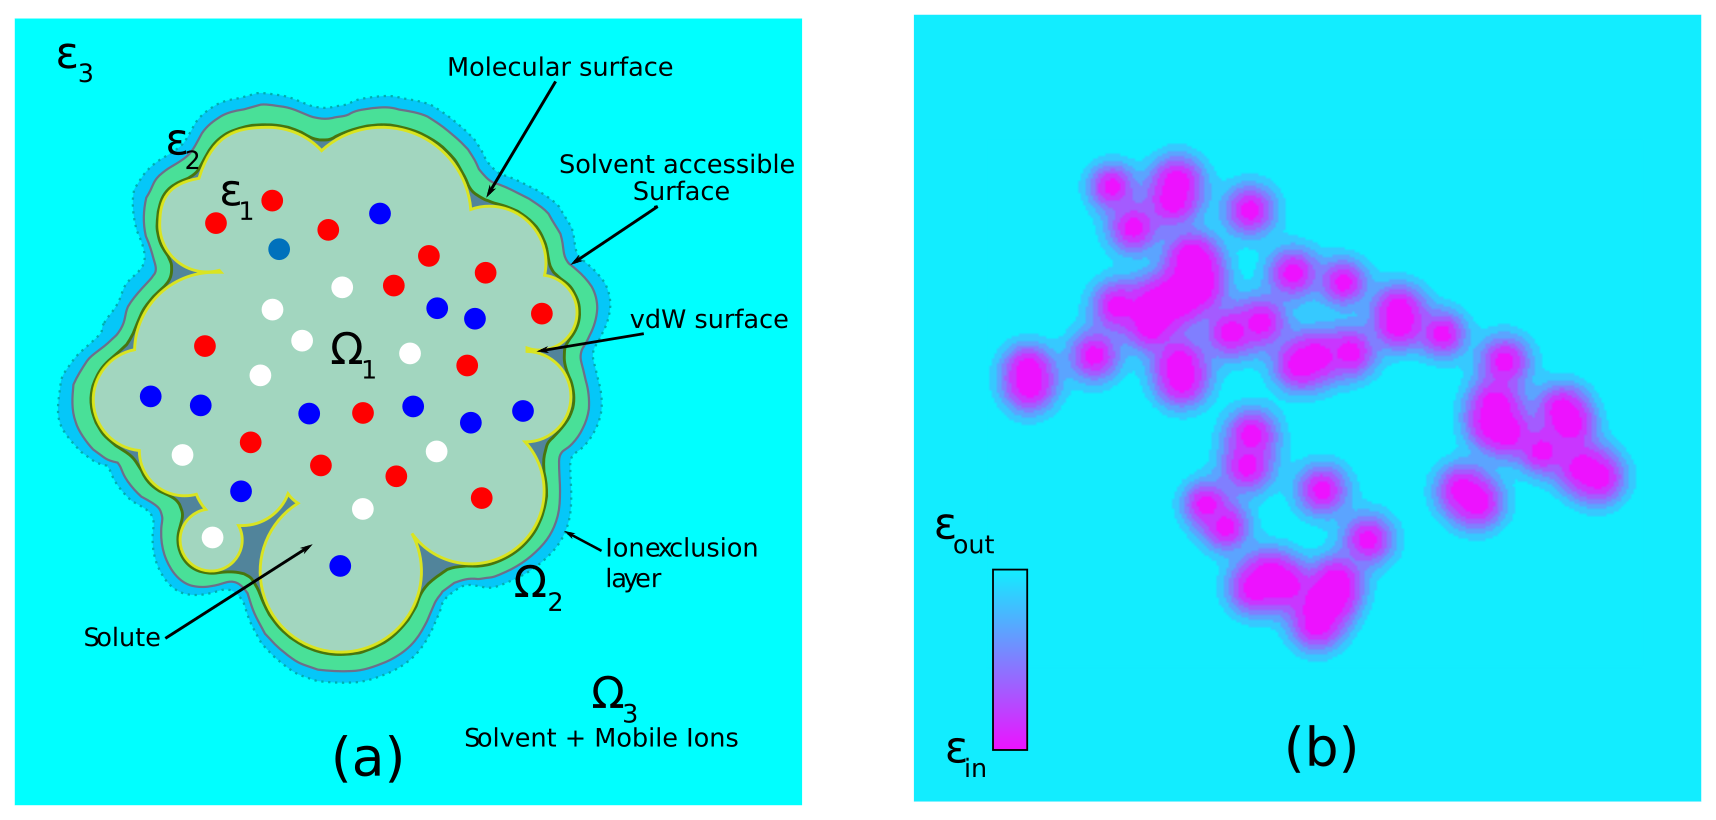
\includegraphics[width=0.95\linewidth]{Figure_1.png}
\caption{\textbf{(a)} Schematic presentation of space partitioning in case of traditional two-dielectric model. In each of these partitions, different differential equation is solved. The domain, which is essentially the 3D space containing the macromolecule(s) and the solvent (with or without ions) is split into three regions labeled as $ \Omega_1$, $ \Omega_2 $ and $ \Omega_3 $. Colored dots are used to represent charge heterogeneity of atoms (red: negatively charged, blue: positively charged and white neutral). \textbf{(b)} Schematic presentation of the dielectric distribution delivered using the Gaussian-based smooth dielectric model (figure shows dielectric function value throughout a slice of a protein). Note that there is no dielectric boundary and even some space regions inside the protein are assigned high dielectric constant.}
\label{fig:Figure_1}
\end{figure*}

The first region of space $ \Omega_1 $, is occupied by the macromolecule(s) and its boundary is defined as the molecular surface. This region is considered as a low dielectric cavity of dielectric constant with permanent charges that belong to the macromolecular atoms. Since it does not contain solvent or mobile ions, its potential distribution ($\phi(\Vec{r})$) is governed purely by Poisson equation, as shown:

\begin{equation}
 \nabla . \left[ \epsilon(\Vec{r})\nabla\phi(\Vec{r}) \right] = -4\pi\rho(\Vec{r})    
\end{equation} 
which can also be rewritten as:
\begin{equation}
\nabla^2\phi(\Vec{r}) = \frac{-4\pi\rho(\Vec{r})}{\epsilon_1} 
\end{equation}
where $ \rho(\Vec{r}) $ denotes the charge density of the fixed charges of the macromolecule(s) in question and $ \epsilon_1 $ is the dielectric constant of macromolecule (typically referred as internal dielectric constant). 

The outer space region or the $ \Omega_3 $ is occupied by the solvent (typically water) which represents a continuum medium with a dielectric value $ \epsilon_3 $. The solvent continuum can also contain mobile ions whose effects are implicitly taken into account using the Boltzmann distribution. The potential distribution in this region is governed by the Poisson-Boltzmann equation (PBE). The charge density due to the mobile ions with concentration M($ \rho_3(\Vec{r}) $) generates a potential distribution that can be expressed as Eqn. \ref{eqn:pbe_1}.

\begin{equation}\label{eqn:pbe_1}
\nabla^2\phi(\Vec{r}) = \frac{-4\pi\rho_3(\Vec{r})}{\epsilon_3} 
\end{equation}

The charge density can be rewritten as Eqn. \ref{eqn:pbe_2}:
\begin{align}\label{eqn:pbe_2}
\rho_3(\Vec{r}) &= M_+ e_c - M_- e_c \nonumber \\
&= e_c M \left(exp\left[ - \frac{e_c\phi(\Vec{r})}{k_BT}\right] - exp\left[  \frac{e_c\phi(\Vec{r})}{k_BT}\right]\right) \nonumber \\
&= e_c M \sinh\left({\frac{e_c\phi(\Vec{r})}{k_BT}}\right)
\end{align}
In these equations, the mobile ion charge density is composed of positive and negative charges (from a monovalent salt) whose corresponding concentrations are $ M_+ $ and $ M_- $. Combining the reformatted mobile ion charge density with PBE, the following can be obtained:

\begin{equation}\label{eqn:pbe_3}
\nabla^2\phi(\Vec{r}) = \kappa^2 \left (\frac{k_BT}{e_c} \right) \sinh\left({\frac{e_c\phi(\Vec{r})}{k_BT}} \right)
\end{equation}

This can be further modified to express the potential in terms of the modified Debye-Hückel parameter ($\kappa^2$).

In the above equations, $ e_c $ is the elementary charge, $ k_B $ is the Boltzmann constant and $ T $ is the absolute temperature.
In between these two regions,  exists the ion-exclusion layer (shown as $ \Omega_2 $) which the mobile ions are not allowed to access. Due to the lack of mobile ions, as well as the absence of permanent solute charges, this region is governed by Laplace’s equation.
\begin{equation}
\nabla^2\phi(\Vec{r}) = 0
\end{equation}
The ion-exclusion layer or the Stern layer has the same dielectric properties as the solvent region or $ \Omega_3 $ (i.e. $ \epsilon_3 $). Therefore, $ \epsilon_2=\epsilon_3 $ . This indicates the role of the molecular surface as the surface that separates two dielectric media. The molecular surface can be constructed using various approaches but they are out of the scope of this article\cite{rocchia2002rapid,chakravorty2019grid,decherchi2013between}. 

Briefly, Van der Waals (vdW) surface is the surface made of atomc vdW surfaces exposed to the solvent. If one runs a water probe, considered to be sphere with radius 1.4 \text{\AA}, and follow the center of the probe, the resulting surface is termed solvent accessible surface (SAS). Moving SAS 1.4 \text{\AA} towards vdW surface results in molecular surface. Finally, the ion accessible surface, which defines Stern layer, is the surface made of ions centers, represented as sphere with typical radius of 2.0 \text{\AA}.

\subsubsection{Space partitioning with the Gaussian-based smooth dielectric model}
The Gaussian-based smooth dielectric model is designed to deliver a continuous distribution of dielectric values in space as opposed to representing it as a union of two media with distinct dielectric constants. 
The smooth distribution reflects the effect of restrictions on the mobility of the macromolecular and solvent regions on their polarizability or the dielectric value. The distribution is assigned based on the macromolecular atomic packing density in a given region. Its formulation ensures that the dielectric value is the lowest ($ \epsilon_{in} $) at the center of the macromolecular atoms and is the highest ( $ \epsilon_{out} $ ) in the bulk. Through this assignment, regions close to the macromolecular atom centers attain a lower dielectric value and those farther away from the macromolecule attain a higher value. Overall, buried or highly densely packed regions of the system feature a lower dielectric value than those which are less packed (details are provided in refs\cite{chakravorty2019grid,decherchi2013between}). This is illustrated in Figure \ref{fig:Figure_1}b.


The key feature of Gaussian-based smooth dielectric functions are that the strict surface (like the molecular surface shown in Figure \ref{fig:Figure_1}a) is replaced by a smooth transition of the dielectric values from the macromolecular interior $ \Omega_1 $ to the bulk $ \Omega_3 $ as shown in Figure \ref{fig:Figure_1}. The transient values of the dielectric at the solute-solvent interface collectively reflect the increased polarizability of solvent exposed atoms of the macromolecule (compared to those in the core regions) and decreased polarizability of the solvent in their vicinity (compared to those in the bulk). This occurs by virtue of the solute-solvent interactions that play a critical role in balancing the effects of (de)solvation and intramolecular interactions of the solvent exposed macromolecular atoms. 
Due to the continuous dielectric distribution, a clear distinction of macromolecular and solvent regions is no longer necessary and therefore, the same differential equation (PE or PBE) can be used homogeneously. However, the lack of a dielectric boundary invites a modification in the way by which the screening effect of mobile ions is taken into account. In the traditional two-dielectric approach, the presence of a mobile ion at a point in space (depending on its accessibility) is guided by the electrostatic potential at that point which is expressed using a Boltzmann distribution function (Eqn. \ref{eqn:pbe_2}). In the Gaussian-based approach, an additional penalty term is added to its potential energy at any point in space (for more details see Ref\cite{jia2017treating}). The penalty term is based on the Born-formalism of the energy of transfer of a centrosymmetric ion across two dielectric media. In the case of the Gaussian-model, the penalty term, $ \Delta G_{penalty} $, is the energy of transfer of an ion of valence $ z $ and Van der Waals radius $ R $ from the solvent (with dielectric $ \epsilon_2 $) to a point  (with dielectric $ \epsilon(\Vec{r})$) and is expressed in SI units as:

\begin{equation}
\Delta G_{penalty} = \frac{N_Az^2e_c^2}{8\pi\epsilon_0 R} \left( \frac{1}{\epsilon(\Vec{r})} - \frac{1}{\epsilon_2} \right)
\end{equation}

$ N_A $ is the Avogadro number and $ \epsilon_0 $ is the value of permittivity of vacuum. When included with the PBE, the modification renders the following form:

\begin{equation}
\nabla^2\phi(\Vec{r}) = \kappa^2 \left (\frac{k_BT}{e_c} \right) \sinh\left({\frac{e_c\phi(\Vec{r})}{k_BT}} \right) e^{-\frac{\Delta G_{penalty}}{k_B T}}
\end{equation}

In Figure \ref{fig:plot_saltation_penalty}, the penalty term as a function of position is shown for a solute with a very simple geometry (one sphere of 2 \text{\AA} radius). As one approaches the vicinity of the solute, the penalty increases dramatically, ensuring that the mobile ions cannot penetrate in the regions dominated by solute’s dielectric values. Farther out in the bulk, the penalty term diminishes to zero, thus retrieving the properties of the traditional 2-dielectric approach.

\begin{figure}[hbt!]
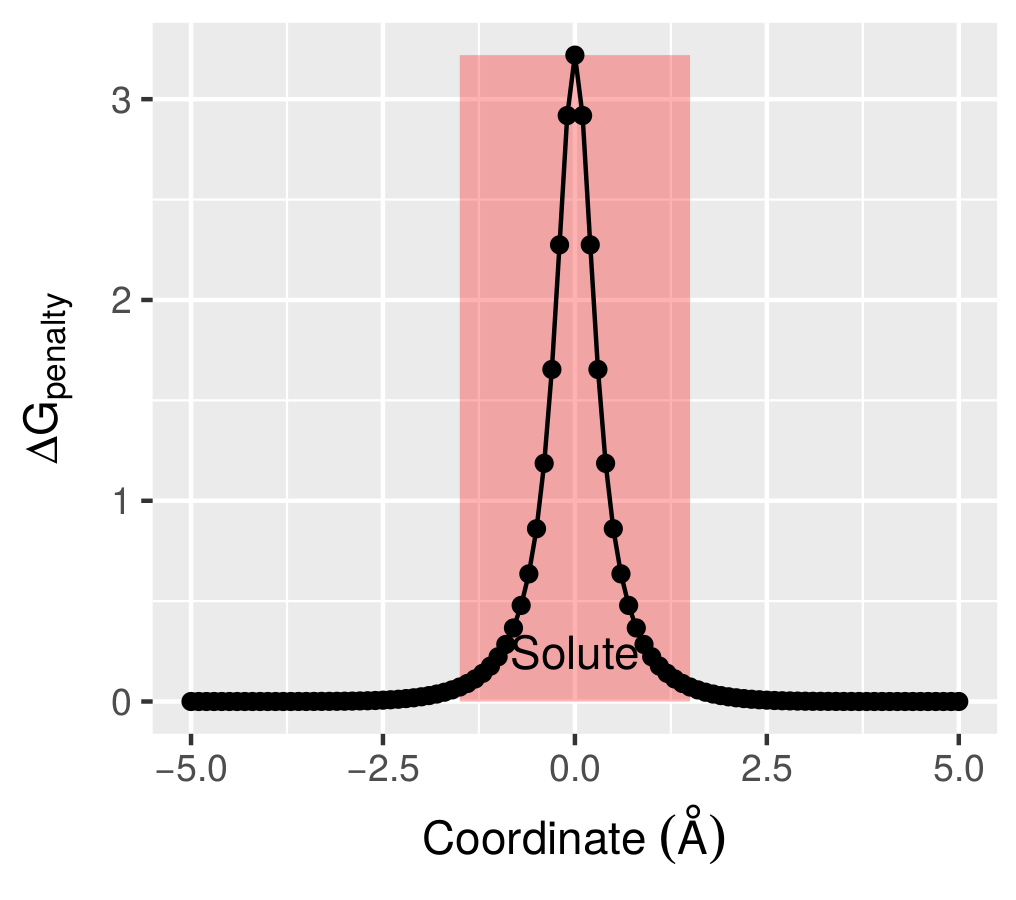
\includegraphics[width=\linewidth]{Figure_2.png}
\caption{The penalty term shown as a function of position along a 1D axis without loss of generality. The solute is centered at the origin and its bounds are shown by the shaded region.}
\label{fig:plot_saltation_penalty}
\end{figure}

\subsubsection{Finite difference algorithm}
The Poisson-Boltzmann equation is a non-linear $2^{nd}$ order differential equation that is typically solved using numerical schemes since analytical solutions are only possible for cases with very simple geometry. Inhomogeneity of charge distribution and complex geometrical features are prerogative of biomolecules, therefore, different methods of numerically solving the PBE for biomolecular systems have been developed \cite{klapper1986focusing,davis1989solving,cortis1997numerical,baker2001electrostatics,shestakov2002solution,miertuvs1981electrostatic,totrov2001rapid,lu2009adaptive}. 
DelPhi solves the PBE using the finite difference (FD) algorithm. The approach rests on discretization of the entire space, $ \Omega=(\Omega_1 \cup \Omega_2 \cup \Omega_3)$, into a set of adjacent cubes, all of the same side length. Along each of the three Cartesian orthogonal directions, an identical number of these cubes are placed and their union forms a larger cube which is also referred to as the computational box. Points where two or more cubes meet are known as the grid points and they are the locations where the electrostatic potentials and electric fields are determined.  Between two adjacently placed grid-points, a mid-point is located where the dielectric values are assigned. Collectively, the grid-points and mid-points are all placed within the bounds of the computational box. Figure \ref{fig:grid-scheme-representation}, provides an illustration of this discretization and a computational box with ‘$ M $’ cubes per side, each with a side length of ‘$ h $’. 

\begin{figure*}
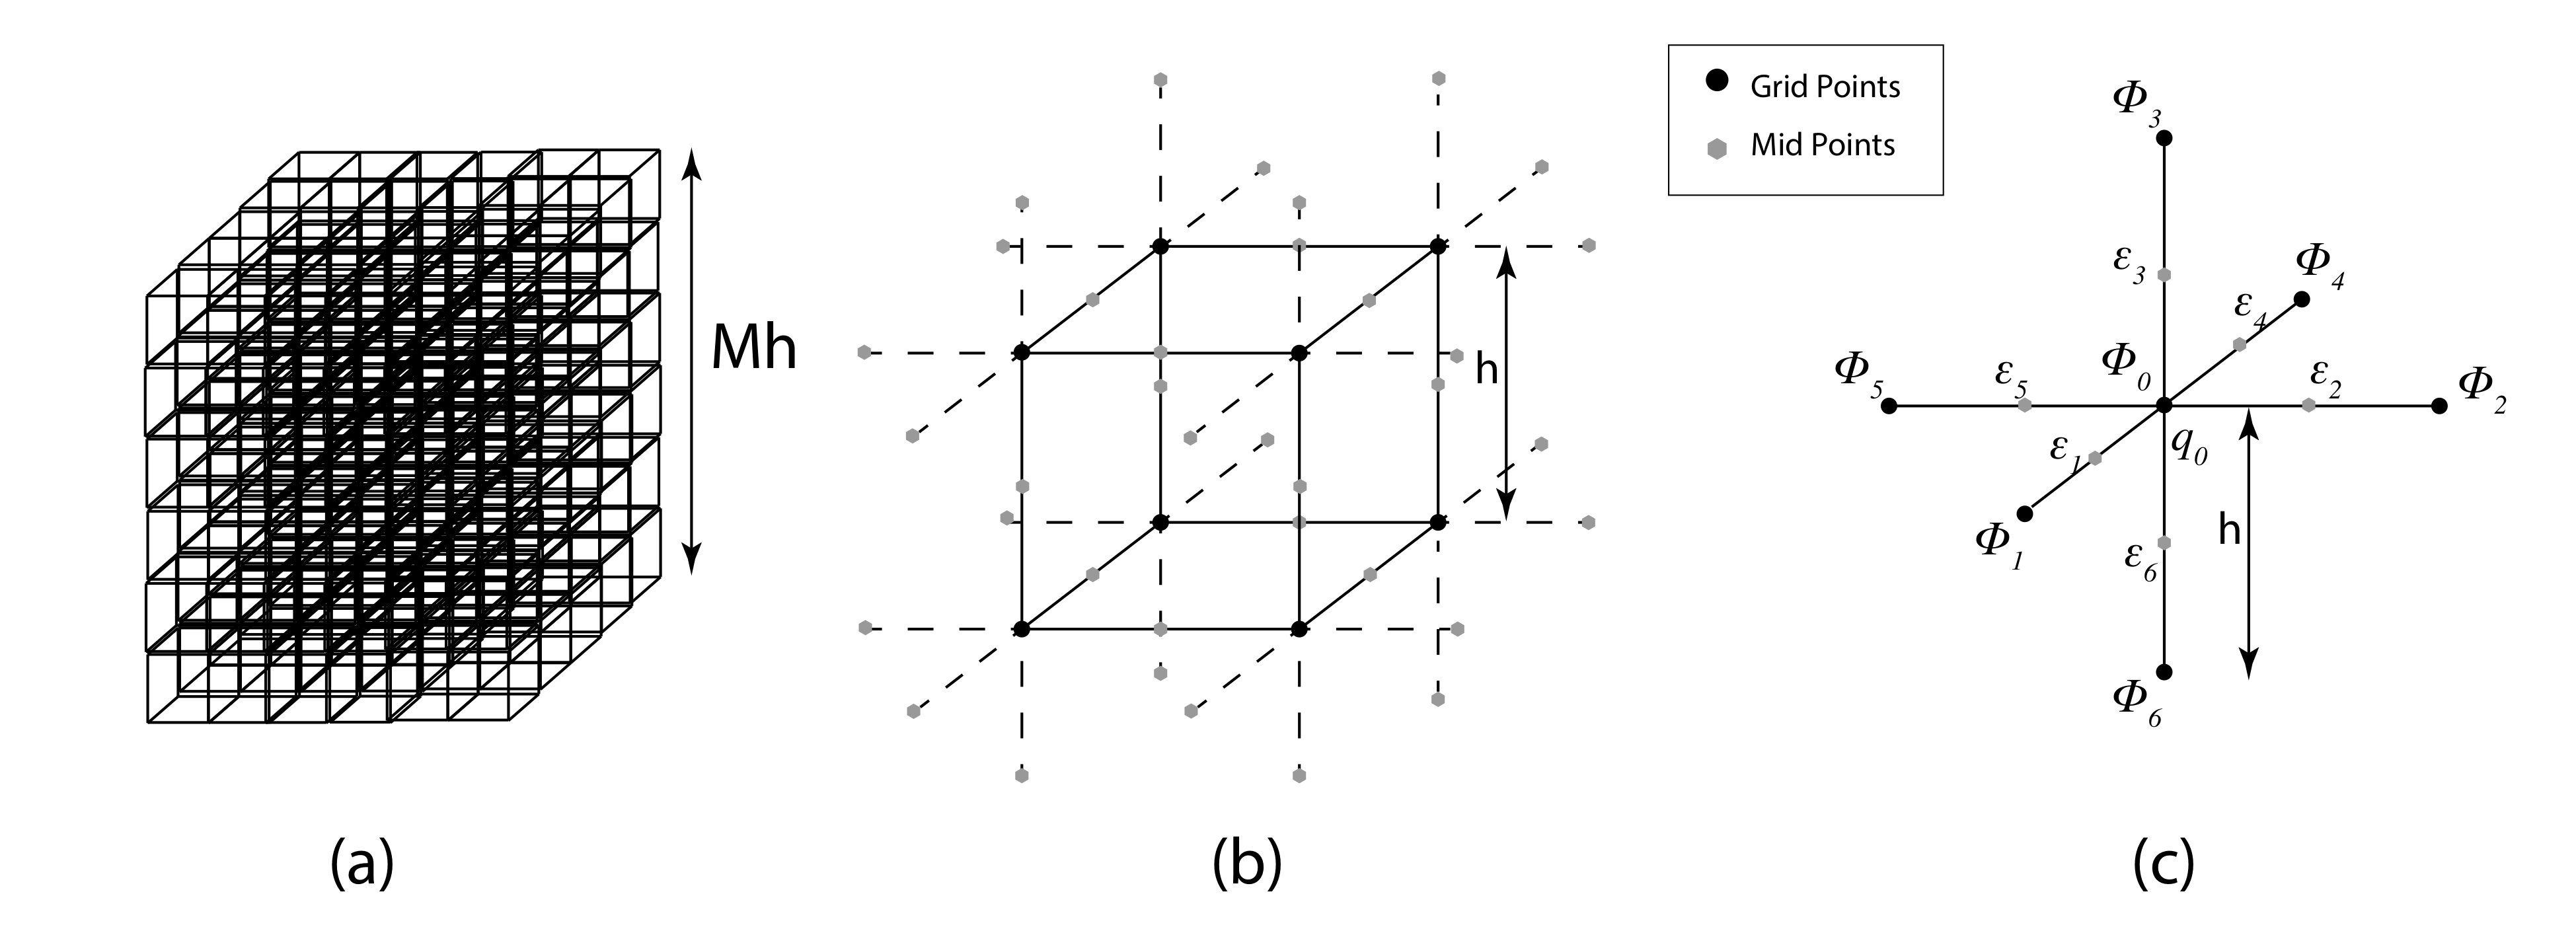
\includegraphics[width=0.95\linewidth]{Figure_3.png}
\caption{Discretization of the space containing the solvated biomolecule. For the finite-difference approach of solving the PBE, DelPhi divides the total space by adjacently placing equal numbers of cubes, each of side length ‘h’, along all the three Cartesian orthogonal directions as shown in \textbf{(a)}. The vertices of a cube are known as the grid-points and are shown in \textbf{(b)} using solid black points. The points in between two adjacent grid-points are called the mid-points where the values of dielectric constants are assigned. They are shown using grey points in \textbf{(c)}.}
\label{fig:grid-scheme-representation}
%% If the optional argument in the square brackets is ``none'', then the caption *will not appear in the main figure at all* and only the full caption will appear under the supplementary figure at the end of the manuscript.
\end{figure*}
 
Instead of solving different variants of the differential equation like the PE and PBE (as mentioned above) in the different partitions or subdomains of the computational box, an iterative protocol based on the integral form of these equations is executed to compute the potential values at each grid-point. To do so, a position dependent formulation of the dielectric values ($ \epsilon $) and the modified Debye-Hückel parameter ($ \kappa $) is used. 

\begin{equation}
  \epsilon(\Vec{r}) = \left \{
  \begin{aligned}
    &\epsilon_1; && \Vec{r} \in \Omega_1 \\
    &\epsilon_2 (=\epsilon_3) ; && \Vec{r} \in \Omega_2 \cup \Omega_3
  \end{aligned} \right.
\end{equation}

\begin{equation}
  \kappa(\Vec{r}) = \left \{
  \begin{aligned}
    &0; && \Vec{r} \in \Omega_1 \cup \Omega_2 \\
    & \sqrt{\epsilon_3}\kappa ; && \Vec{r} \in \Omega_3
  \end{aligned} \right.
\end{equation}

This ensures a consistent formulation of the non-linear PBE in the whole domain $ \Omega = \Omega_1 \cup \Omega_2 \cup \Omega_3 $ in the following manner:

\begin{equation}
    \nabla.\left[\epsilon(\Vec{r})\nabla\phi(\Vec{r})\right] = \Bar{\kappa}(\Vec{r})\frac{k_BT}{e_c}\sinh{\frac{e_c\phi(\Vec{r})}{k_BT}} - 4\pi\sum_{i} {q_i \delta(\Vec{r} - \Vec{r_i})}
\end{equation}

For every atom $ i $ of the macromolecule, its charge and position are denoted using $ q_i $ and $ \Vec{r_i}$. The hyperbolic sine function can be approximated using the first term of its Taylor series expansion to yield a simplified linearized form of the PBE, or the linear PBE. This is expressed as:
\begin{equation}
\nabla . \left[ \epsilon(\Vec{r})\nabla\phi(\Vec{r})\right] = \Bar{\kappa}(\Vec{r})\phi(\Vec{r}) - 4\pi\sum_{i} {q_i \delta(\Vec{r} - \Vec{r_i})}
\end{equation}
In the case of the Gaussian-based smooth dielectric model, subdomains do not exist. As a result,  dielectric function and the modified Debye-Hückel parameter are continuous functions in space. In presence of a salt in the solution, the non-linear acquires the following forms:
\begin{equation}
\nabla.\left[\epsilon(\Vec{r})\nabla\phi(\Vec{r})\right] = \left[
    \begin{aligned}
    & \Bar{\kappa}(\Vec{r})\frac{k_BT}{e_c}\sinh{\left(\frac{e_c\phi(\Vec{r})}{k_BT}\right)}e^{-\left(\frac{\Delta G_{penalty}}{k_BT} \right)} \\
    &- 4\pi\sum_{i} {q_i \delta(\Vec{r} - \Vec{r_i})}
\end{aligned}
\right]
\end{equation}
The linearized version of the PBE in case of the Gaussian-based dielectric model in presence of non-zero salt concentration can be expressed as:
\begin{equation}
\nabla . \left[ \epsilon(\Vec{r})\nabla\phi(\Vec{r})\right] = \Bar{\kappa}(\Vec{r})\phi(\Vec{r})e^{-\left(\frac{\Delta G_{penalty}}{k_BT} \right)} - 4\pi\sum_{i} {q_i \delta(\Vec{r} - \Vec{r_i})}
\end{equation}

By performing a finite volume integration of the above linear PBE and projecting the results in the discretized space, one can derive a numerical formula that establishes a relation of the electrostatic potential, $ \phi_0 $, on a grid-point with that of the six of its neighboring grid-points (see Figure \ref{fig:grid-scheme-representation}(c)). The value also depends on the charge ($ q_0 $) and the modified Debye-Hückel parameter ($ \Bar{\kappa}^2 $) on the grid-point and also on the dielectric values at the six midpoints surrounding it. The numerical formula has the following form:
\begin{equation}
    \phi_0 = 
    \left[ 
        \frac{\sum_i^6{\epsilon_i\phi_i } + 
                \frac{4\pi q_0}{h}
             }
             {\sum_i^6{\epsilon_i} + \Bar{\kappa}^2h^2}
    \right]
\end{equation}
When the Gaussian-based smooth dielectric model is invoked, the FD formula remains the same expression except that it incorporates a space dependent penalty term imposed on the mobile ions. The modified expression has the following form:

\begin{equation}
    \phi_0 = 
    \left[ 
        \frac{\sum_i^6{\epsilon_i\phi_i } + 
                \frac{4\pi q_0}{h}
             }
             {\sum_i^6{\epsilon_i} + \Bar{\kappa}^2h^2e^{-\left(\frac{\Delta G_{penalty}}{k_BT}\right)}}
    \right]
\end{equation}
Regardless of the dielectric model, the computation of the potential is initiated by specifying  some boundary condition on the potential (typically the potential at the edges of the computational box). Following this, the FD based numerical formula iteratively updates the potential at any given grid point until the values converge. Convergence itself is defined using certain measures of tolerance which are not discussed here. 
 
\subsection{Energy partitioning}
Once the potential distribution is calculated, the next step in DelPhi algorithm is to compute the electrostatic energies. Based on the original paper of Sharp and Honig\cite{sharp1990electrostatic}, see also\cite{rocchia2001extending}, the energy components are:
Grid energy
\begin{equation}
    G_{grid} = 0.5 \left[ \sum_i^{grids}{p_i\phi_i} \right]
\end{equation}
where $ p_i $ is the charge of grid point `$ i $' and $ \phi_i $ is the grid potential at the same grid point. Note that this energy term contains artificial components due to the real charge partitioning over the grid points. Direct usage of $ G_{grid} $ is not appropriate, only grid energy difference can be used.

The total electrostatic energy of the system can be decomposed into three energy terms\cite{rocchia2001extending}, Coulombic, polar solvation and saltation energies. In case of traditional two-dielectric model, this is described in Ref. \cite{rocchia2001extending}. Thus, the Coulombic term is the product between real charges over the distance, and it is computed via Coulombic formula:

\begin{equation}
    G_{Coul} = 0.5 \left[ \sum_i^{\text{number of charges}}{\frac{q_i q_j}{\epsilon_{in}r_{ij}}} \right]
\end{equation}	
where $ q_i $ are the real charges, $r_{ij} $ is the distance between charge `$i$' and `$j$', and $ \epsilon_{in} $ is the internal dielectric constant. 

The second energy term is the polar solvation energy, which in DelPhi is called ``corrected reaction field energy'', or ``$ G_{rxn} $''. Following original development due to Anthony Nicholls, this energy is calculated via induced charges on the molecular surface. The induced charges ($ \sigma_j $) are calculated using electrostatic potential distribution over the molecular surface. The $ \sigma_j $ are obtained via Gauss's Law at the corresponding grid point and then projected to the molecular surface (more details are provided in \cite{rocchia2001extending}). Thus, 

\begin{equation}\label{eqn:G_rxn}
    G_{rxn} = 0.5 \left[ \sum_{i, j}^{\text{number of charges/induced charges}}{\frac{q_i \sigma_j}{\epsilon_{out}r_{ij}}} \right]
\end{equation}
where $ \sigma_j $ are induced surface charges. 

The third term represents the energy of interactions between permanent charges and mobile ions. Formally it could be described by a formula similar to Eqn. \ref{eqn:G_rxn}, where instead of induced charges one takes excess ion density. However, this approach was abandoned in the newest DelPhi version because it is very slow and requires small “percent fill”. Instead, we recommend using grid energy difference between runs with salt and without salt. 

Finally, if one invokes non-linear PBE, two additional energy terms should be added to the total electrostatic energy. Following the work of Sharp and Honig\cite{sharp1990electrostatic}, they are termed ``osmotic pressure'' and ``electrostatic stress''.


\section{Prerequisites}

DelPhi uses FD algorithm to solve the PBE and thus to deliver the electrostatic potential distribution. The first step in the algorithm requires that one provides a coordinate file of the biomolecules and nano-objects in PDB or PQR formats. In the second case, the input PQR file provides the coordinates of all atoms along with their radii and charges. In the first case, the user needs to provide two additional files, the ``size'' and ``charge'' files. These files contain information about the atomic radii and charges. If PDB format file is provided, then DelPhi matches the names of the atoms/residues toward the names/radii in the corresponding ``size'' and ``charge'' files and thus generates information for each atom position, radius and charge (note that if the PDB file contains atomic names/residues not available in the corresponding ``size'' and ``charge'' files, then DelPhi will generate warning message prompting the users that these names/residues are not recognized). Once the atomic coordinates and radii are available, DelPhi builds grid presentation of the geometrical and dielectric properties of the system. By default, it is done by positioning the macromolecule(s) geometrical center at the center of the computational box and using ``scale'', ``grid size'' and ``percent fill''. 

\begin{figure}[hbt!]
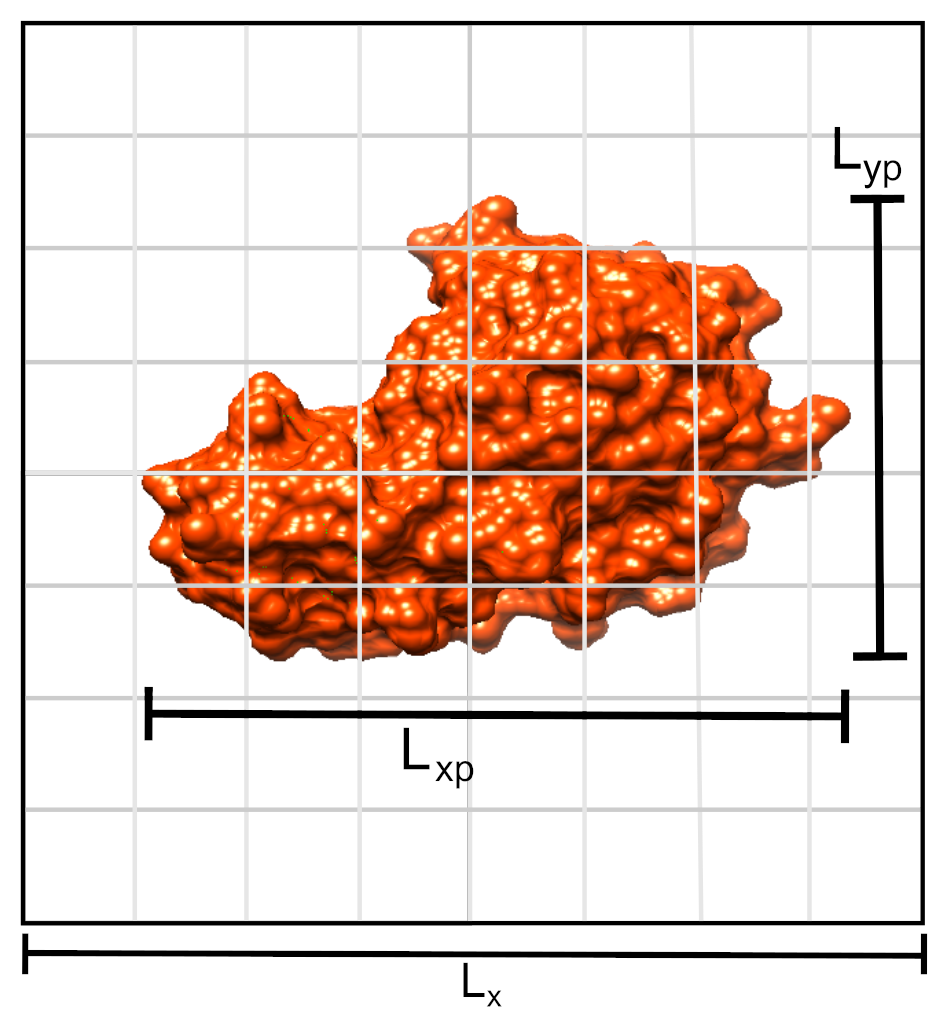
\includegraphics[width=\linewidth]{Figure_4.png}
\caption{The schematic representation of relationship between ``percent fill'' (\ttvar{perfil}), ``grid size'' (\ttvar{gsize}), and \ttvar{scale}. The parameter \ttvar{gsize} decides number of grid lines in each direction e.g. \ttvar{gsize} is 9 in given cartoon. The parameter \ttvar{scale} decides number of grid lines per \text{\AA}. If we assume \ttvar{perfil} $ pf\% $ and maximum dimension in X-, Y- directions be $ L_{xp} $ \text{\AA} and $ L_{yp} $ \text{\AA} as shown in cartoon, then the size of the grid box $ L_x $ in \text{\AA} is computed using relation $ L_x = \frac{max(L_{xp}, L_{yp}) \times 100}{pf} $. The value of \ttvar{scale} in this case would be $ \ttvar{scale} = \frac{L_x}{\ttvar{gsize}} = \frac{L_x}{9} $.}
\label{fig:perfil-gsize-scale}
\end{figure}

Note that these three parameters, ``scale'', ``grid size'' and ``percent fill'' are interdependent (Figure \ref{fig:perfil-gsize-scale}). Only two are needed. Users are advised to use ``scale'' and ``percent fill'' (\ttvar{perfil}) and to let DelPhi decide the ``grid size'' (\ttvar{gsize}). In the traditional two-dielectric model, the computational box is split into low dielectric cavities occupied by macromolecule(s) and water phase and appropriate dielectric constant values are assigned to the mid-point belonging to the corresponding phases. In the Gaussian model, coordinates and radii are used to construct a smooth Gaussian-based dielectric function for the entire computational box without distinguishing the macromolecule(s) from the water phase (for mode details see Refs \cite{li2014modeling,li2013dielectric}). Once this is completed, DelPhi initiates FD iterations to compute electrostatic potential distribution and to calculate the corresponding energy, as it will be outlined below. Several practical advice about DelPhi parameters are given here:

\begin{enumerate}
    \item How to decide on geometry? One wants the macromolecule(s) to occupy significant percent of the computational box space so the calculations to focus on important part of the system. However, doing modeling with very high ``percent fill'' may result in positioning some of the macromolecule(s) atoms too close to the edges of the computational box and thus to introduce an error. We recommend ``percent fill'' of about 70\%. 

    \item How to decide on the ``dielectric constants''? Most of the modeling involves biological macromolecules in water, so natural choice of the dielectric constant of solvent is the dielectric constant of bulk water, typically taken as 80. Regarding internal dielectric constant: (a) in case of traditional two-dielectric model, one selects the value of internal dielectric constant depending on the modeling protocol. If one models rigid structures or snap shots taken from MD simulations, the internal dielectric constant value is typically set to 1.0. However, in other modelings one may select values that are higher with the goal to match experimental data or to mimic for conformational flexibility not accounted in the protocol (b) in case of smooth Gaussian-based dielectric function, one selects the reference value of internal dielectric constant based on benchmarking (see refs\cite{li2014modeling,li2013progress,wang2015pka,wang2015delphipka} for more details).  

    \item Criteria for convergence. The FD algorithm is iterative and its convergence is monitored via several parameters as ``maxc'', which is the largest change of the potential from iteration `i' to `i+1'; or ``rmsc'', which root mean square change of the potential. In both cases, it is recommended to use small, but reasonable criteria of 0.0001. 

    \item Linear versus non-linear PBE. DelPhi allows the user to select what form of PBE to be solved: linear or non-linear. Solving non-linear PBE is typically more time consuming and should be avoided if not necessary. Typically, if the system does not have large net charge, there is no need to invoke non-linearity\cite{talley2008electrostatic,chakavorty2016electrostatic}.
\end{enumerate}

\subsection{Background knowledge}
DelPhi takes as an input various files and the corresponding parameters. The most important are the files containing the coordinates of the atoms of the macromolecule(s) and nano-objects. Typically, these files are taken from PDB and often do not have hydrogen atoms. Even more, frequently, structural files deposited in PDB have missing atoms or residues. Because of that, users must first subject their coordinate files to some third-party software to add missing structural information and to assign missing hydrogens. There are many options to do this, including DelPhiPKa\cite{wang2015pka,wang2015delphipka,pahari2018delphipka} and PDB2PQR\cite{dolinsky2007pdb2pqr}. We emphasize on using DelPhiPKa since it allows the protons to be added according to user’s specified pH via adjusting their protonation states of titratable groups. In general, the user can use DelPhi with any structural file provided that the coordinates on the atoms/pseudo-atoms are given along with the corresponding radii and charges. 

As it will be discussed in detail in following sections, the user may have to provide additional PDB-like files either in case of modeling interactions between macromolecules or computing the electrostatic potential at given point(s) in space. 

User responsibility is to select appropriate set of force field parameters. There is no preference regarding force field parameters, however, it is strongly recommended to keep consistence: if structures are energy minimized or subjected to MD simulations with a given force field (Charmm, Amber etc.) the same force field parameters should be used for DelPhi calculations.

\subsection{Software/system requirements}
DelPhi website provides download links to multiple versions (Fortran77, Fortran95 and C++) of the DelPhi program. It is recommended to all users to download the latest C++ version of the DelPhi program to enjoy all features supported by the DelPhi program. DelPhi website also provides precompiled binary executables. However, it is recommended to download the source code and compile the source code in user’s individual environment to generate the executable. Taking the latest DelPhiC++ 8.4.1 as an example, the following software and system requirements must be met in order to successfully compile and run the DelPhi program(s).
\newcolumntype{C}[1]{%
  >{\raggedright\arraybackslash}p{\dimexpr#1-2\tabcolsep}%
}

\begin{table*}[bt!]
\caption{\label{tab:example}DelPhiC++ System requirements}
% Use ``S'' column identifier to align on decimal point
% ``l'' left aligns text in the column
% ``r'' right aligns text in the column
% ``c'' right aligns text in the column
% & separates columns, \\ ends the row.

\begin{tabular}{C{.19\textwidth}C{0.27\textwidth}C{.27\textwidth}C{.27\textwidth}}
\toprule
{Operating System} & {DelPhiC++ (Single-CPU)}  & {DelPhiC++ (Multi-CPU via OpenMP)} & {DelPhiC++ (Multi-CPU via MPI)}\\
\midrule
\multicolumn{1}{l}{Windows XP and above} & 1. Minimalist GNU for Windows (MinGW) \newline
    2. GCC compiler version 5.4.0 and above. &
    1. GCC compiler version 5.4.0 and above with OpenMP support. &
N/A \\
\multicolumn{1}{l}{Mac OS X and above} &
    1. GCC compiler version 5.4.0 or CLANG 7.3.0 and above &
    1. GCC compiler version 5.4.0 or CLANG 7.3.0 and above with OpenMP support &
N/A \\
Linux Distributions such
as Ubuntu 16.4.3 and above &
    1. GCC compiler version 5.4.0 and above. &
    1. GCC compiler version 5.4.0 and above with OpenMP support. &
    
    1. GCC compiler version 5.4.0 and above. \newline
    2. Boost library installed in /usr/include and its path is recognized in the user environment. \newline
    3. latest version of OpenMPI or MPICH \newline  \\
\bottomrule
\end{tabular}
\medskip
\end{table*}

\textbf{Recommendations}: If one computes electrostatics for a relatively small biological macromolecule or nano-object of a size of several hundred Angstroms, typically at resolution “\texttt{scale = 2.0}” the resulting grid size is several hundred grids in one direction. For such cases it is recommended to use either the serial or Open-MP versions. For systems of extremely large size, resulting in a mesh more than 1,000 grids in one direction, it is recommended to use MPI DelPhi version. 

\section{Content and links}

DelPhi source code and stand-alone precompiled executable can be downloaded from \url{http://compbio.clemson.edu/delphi}. The force field parameter files, size and charge files, examples and tutorial can be downloaded from \url{http://compbio.clemson.edu/delphi}. All the example cases discussed in present article with all the required files can be obtained from \githubrepository. All the examples are kept in \ttvar{LiveCoMS_Examples/} directory of the repository. After cloning this repository to local computer, change current directory to \ttvar{LiveCoMS_Examples/} and execute below command once. It will define the \ttvar{$DELPHI_EXE} environment variable in \ttvar{~/.bashrc} file. 

\begin{verbatim}
bash set-delphi-path.sh
\end{verbatim}

Now close your terminal and restart the terminal. Now the user shall be able to perform calculations discussed in all of the examples compiled in directory \ttvar{LiveCoMS_Examples/}. All the paths mentioned in individual sections are relative to this directory.

\subsection{Set of tutorials for DelPhi stand-alone package}
DelPhi reads parameters, instructions and other necessary details from a parameter file. The parameter file contains names of files providing coordinates of biomolecules and if necessary the files with atomic charges and radii. Detailed instructions about the syntax of parameter files are provided in the user manual. Below we describe a set of examples that show the users how to set up parameter and other files to compute various electrostatic quantities. 

\subsubsection{Computing solvation energy} 

In this section, we describe how to calculate electrostatic component of solvation energy, i.e. $ \Delta G_p $ for a single atom and a real protein, as shown in Figure \ref{fig:scheme_polar_solvation}. 

\begin{figure}[hbt!]
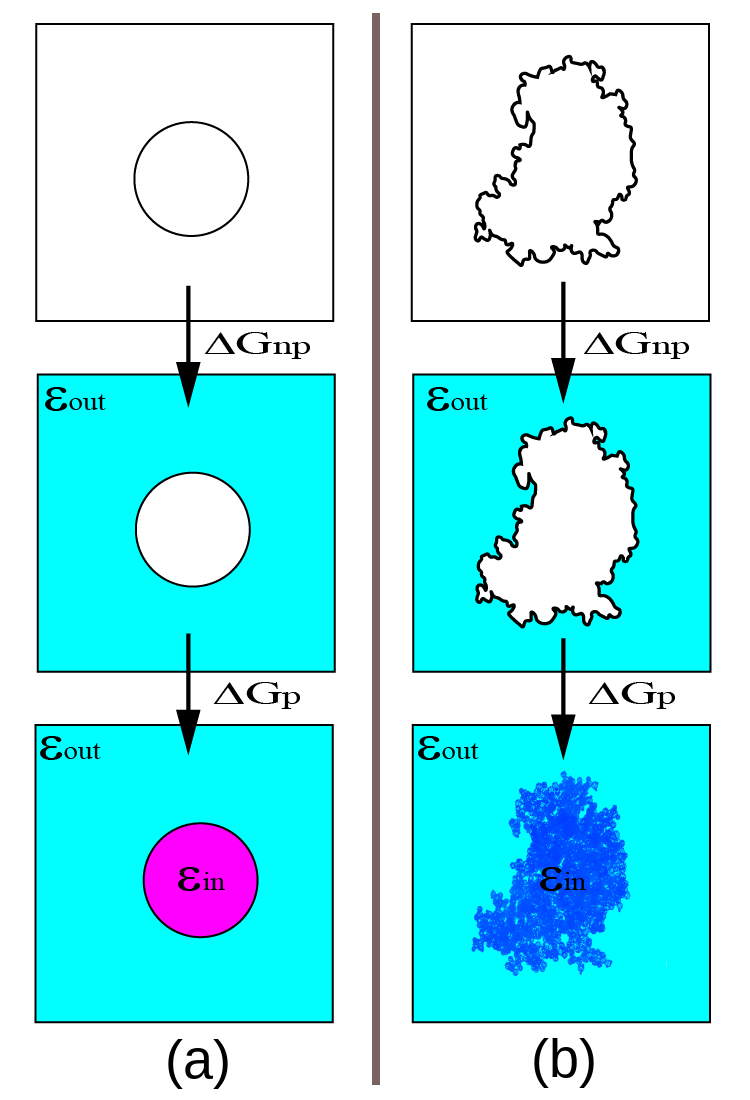
\includegraphics[width=\linewidth]{Figure_5.png}
\caption{The schematic representation of computation of solvation for  \textbf{(a)} a charged sphere and \textbf{(b)} a protein. The solvation of a molecular system consists of two  components, non-polar component $ \Delta G_{np} $ and polar component $ \Delta G_p $. The non-polar components accounts for the energy required to create a cavity to accommodate the molecular system (solute) in the solution or moving solute from gas phase into solvent keeping solute atoms partial charges turned off, and polar component accounts energy required to turn on the partial charges of solute atoms in the solvent.}
\label{fig:scheme_polar_solvation}
\end{figure}

The case of single atom (a charged sphere) is considered because there is an analytical solution via Born formula of charged ion, and the numerical solution provided by DelPhi can be compared with the analytical. In this section, we also provide examples of computing electrostatic solvation energy using traditional two-dielectric model as well as the Gaussian-smooth dielectric function PBE. The corresponding files can be found in directory \ttvar{Example_3.1.1/} and sub directories there in.

We will begin with the simplest case of charged sphere (see \ttvar{Example_3.1.1/Ex1/}) using traditional two-dielectric model. Consider a charged sphere of radius 3 Å carrying a charge +1 e.u. (electron units). Let’s consider that internal and external dielectric constants are 1 and 80, respectively. Thus, the analytical solution is -92.33 kT. DelPhi can be executed using the files provided in above mentioned directories as:

\begin{verbatim}
$DELPHI_EXE param_charged_sphere.prm \
              > charged_sphere.log
\end{verbatim}

After the run is completed, the user can find the corrected reaction field energy from the output information in the log file, which is: 
\begin{verbatim}
Energy > Corrected reaction field energy  : -92.50 kT
\end{verbatim}

Thus, the numerical solution delivered by DelPhi matches the analytical solution. Users are advised to check the sensitivity of results by changing the “scale” parameter. 

Applying Gaussian-based smooth dielectric function approach on the same problem, the charged sphere, results in different polar solvation energy. First, there is no analytical solution since the sphere is no longer hard sphere, but rather a spherical object with smooth dielectric function having minimum value at the center of the sphere and smoothly reaching 80 in bulk solvent. DelPhi can be executed with this example as:

\begin{verbatim}
$DELPHI_EXE param_charged_sphere_gauss.prm \
              > charged_sphere_gauss.log
\end{verbatim}

The calculated polar solvation energy is in the log file:

\begin{verbatim}
Energy> Corrected reaction field energy : -211.20 kT
\end{verbatim}

Note that the computed energy depends on two parameters: \texttt{sigma=0.9} and \texttt{srfcut=20.0} and any change of these parameters will result in a different energy. 

The other example of how to calculate polar solvation energy of a protein, all the related files are kept in the directory \ttvar{Example_3.1.1/Ex2/}. The DelPhi run for computing it via traditional two-dielectric approach can be initiated using command below:

\begin{verbatim}
$DELPHI_EXE param_protein.prm > protein.log
\end{verbatim}

After the run, the user can find the output information in the log file: 

\begin{verbatim}
Energy> Corrected reaction field energy : -1005.07 kT
\end{verbatim}

Similarly, modeling the same protein with Gaussian-based smooth dielectric function can be done by invoking DelPhi and appropriate parameter file as:

\begin{verbatim}
$DELPHI_EXE param_protein_gauss.prm \
              > protein_gauss.log
\end{verbatim}

After the run is completed, one finds the output information in the log file: 

\begin{verbatim}
Energy> Corrected reaction field energy : -3583.05 kT
\end{verbatim}

Note that "corrected reaction field energy" values are quite different for traditional two-dielectric and Gaussian-based methods. This is not surprising, since traditional two-dielectric approach is intending to deliver solvation energy of a rigid molecule, while Gaussian-based method intends to mimic the effects of conformational changes.

\subsubsection{Computing "saltation energy"}

The schematic representation of the process of computing saltation energy is shown in Figure \ref{fig:scheme_saltation}. In order to compute the saltation energy of a system at a given salt concentration two different DelPhi runs are required, first to compute the $ \Delta G_{z} $ the energy of the system at zero salt concentration in the solvent and second to $ \Delta G_{nz}([salt]) $ , the energy at the given salt concentration $[salt]$, here energy refers to grid energy of the DelPhi. Then saltation energy is $ \Delta\Delta G_{nz}([salt]) = \Delta G_{nz}([salt]) - \Delta G_{z}$. In this section we will discuss two cases (I) saltation of a spherical charge whose analytical solution is also known and DelPhi results will be compared against it, and (II) saltation of a real protein (barnase-barstar complex).
\newline
\newline

\begin{figure}[hbt!]
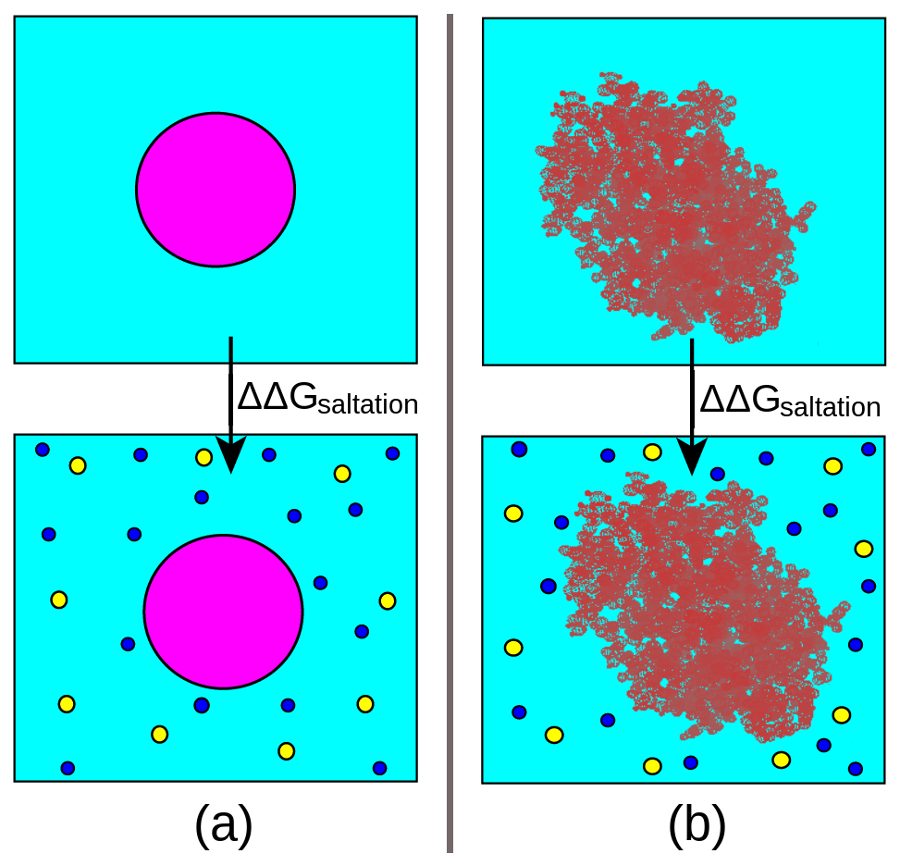
\includegraphics[width=\linewidth]{Figure_6.png}
\caption{Schematic representation of process of computing saltation energy. In the figure spherical charge is shown as circle in panel \textbf{(a)} and protein with cartoon representation in \textbf{(b)}, blue and yellow dots in boxes at bottom represent positive and negative ions of the salt. The saltation energy represents energy required to transfer the solute from a pure solvent (no salt) to a solution with salt concentration [salt] M.}
\label{fig:scheme_saltation}
%% If the optional argument in the square brackets is ``none'', then the caption *will not appear in the main figure at all* and only the full caption will appear under the supplementary figure at the end of the manuscript.
\end{figure}


\textbf{(I) Saltation energy of a charged sphere}

Here, we refer energy of interaction between equilibrated mobile ions and permanent charges of the solute as "saltation energy". In case of a charged sphere one can calculate the energy of interaction between the charged sphere and surrounding ions using Eqn. \ref{eqn:saltation_23}.

\begin{equation}
I_B = \frac{e_c^2}{(4\pi\epsilon_0\epsilon_{ext}k_BT)} 
\end{equation}
\begin{equation}
\kappa^{-1} = \sqrt{\left(\frac{\epsilon_0\epsilon_{ext}k_BT}{2 \times 10^3N_Ae_c^2 C} \right)}
\end{equation}
\begin{equation}
\Delta G_{nz}([salt], R) = \frac{1}{2}k_B T \left(\frac{Q}{e_c}\right)^2\frac{I_B \kappa^{-1}}{R(R+\kappa^{-1})}
\end{equation}
\begin{equation}
\Delta G_z(R) = \frac{1}{2}k_B T \left(\frac{Q}{e_c}\right)^2\frac{I_B}{R}
\end{equation}
\begin{equation}\label{eqn:saltation_23}
\Delta\Delta G_{nz}([salt]) = \Delta G_{nz}([salt], R) - \Delta G_z(R)
\end{equation}

where $I_B$ is Bjerrum length, $ C $ is ionic strength in M, $ k_B $ is Boltzmann constant, $ T $ is absolute temperature, $ e_c $ is the electronic charge, $ \kappa^{-1} $ is Debye length, $ \epsilon_0 $ is the electric permittivity of free space, $ \epsilon_{ext} $ is the external dielectric constant of the medium, $ R $ is the radius of charged sphere, $ \Delta G_{nz}([salt], R) $ is electrical energy of charged sphere in solvent with salt, $ \Delta G_z(R) $ is the electrical energy of charged sphere in solvent without salt, $ \Delta\Delta G_{nz}([salt]) $ is the saltation energy of charged sphere.

Thus, using the following parameters R=10 Å, internal and external dielectric constants 1 and 80, respectively,  and varying salt concentration from 0.02 M until 0.2 M, the analytical and numerical (using DelPhi) solutions are calculated and plotted against logarithm of salt concentration (Figure \ref{fig:plot_saltation_spherical_charge}). For example, with salt concentration 0.02 M and external dielectric constant 80 the analytical and numerical (using DelPhi) solutions for the saltation energy of the charged sphere are -2.77 kT and -2.92 kT, respectively.

\begin{figure}[hbt!]
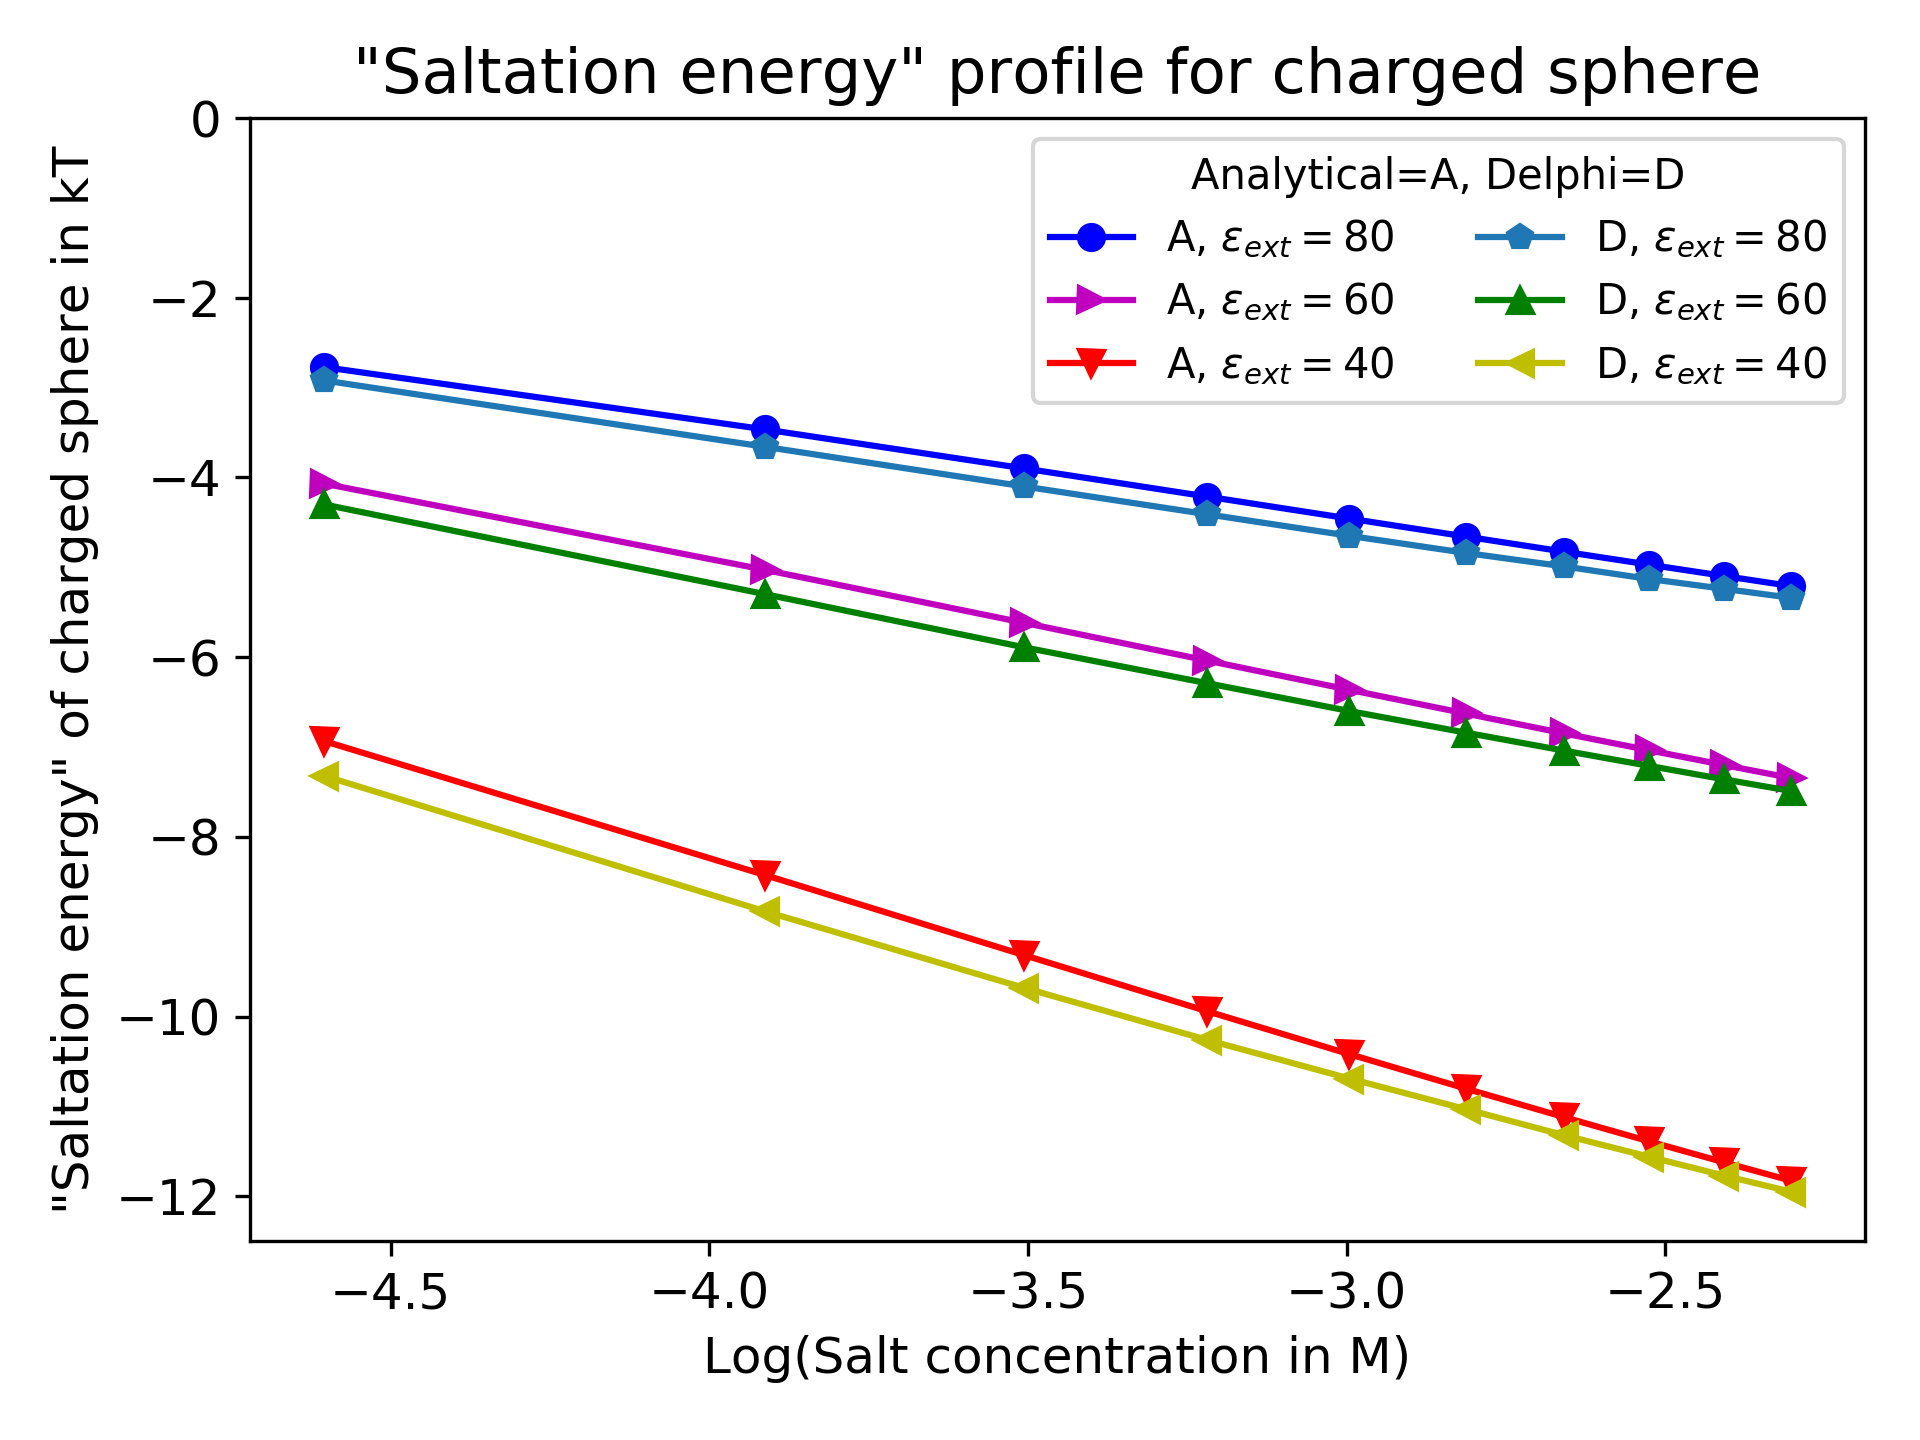
\includegraphics[width=\linewidth]{Figure_7.png}
\caption{Analytical and DelPhi result for the saltation energy of the charged sphere in different salt concentration and different external dielectric constants.}
\label{fig:plot_saltation_spherical_charge}
%% If the optional argument in the square brackets is ``none'', then the caption *will not appear in the main figure at all* and only the full caption will appear under the supplementary figure at the end of the manuscript.
\end{figure}


These calculations are done by using prepared files in the folder \ttvar{Example_3.1.2/Ex1/}. To run these examples on your own machine, execute python script \ttvar{Run-saltation-charged-sphere.py} as:

\begin{verbatim}
python3 Run-saltation-charged-sphere.py
\end{verbatim}

On running this script, the above mentioned analytical and DelPhi calculations are performed and plot (\ttvar{plot-salt-ele-sphere.png}) and csv(\ttvar{saltation_charged_sphere.csv}) file containing results are created. As is shown in the Figure \ref{fig:plot_saltation_spherical_charge}, the calculated “saltation energy” is in excellent agreement with the analytical solution.
\newline

\textbf{(II) Saltation energy of a protein}

In present case, we will discuss computing the "saltation energy" of a real protein (barnase-barstar complex; PDB Id: 1BRS). This example is given as \ttvar{Example_3.1.2/Ex2/} in the example suit. As discussed in the previous section, to compute the saltation energy at a given salt concentration, we are required to obtain the total grid energy for the molecular system at non-zero salt concentration and zero salt concentration, followed by taking their difference. Again, in this case we have computed saltation energy for this system at varying salt concentrations from 0.02M until 0.2M in steps of 0.02M and same way for three different external dielectric (80, 60, and 40) mediums. The python script \ttvar{Run-saltation-protein.py} provided in the directory creates parameter files for the DelPhi run, executes it and parses results to obtain saltation energy which is then written to file \ttvar{saltation_protein.csv}. In addition it also plots saltation energy vs. $log([salt])$ where $ [salt] $ is salt concentration in $ M $. 

\begin{figure}[hbt!]
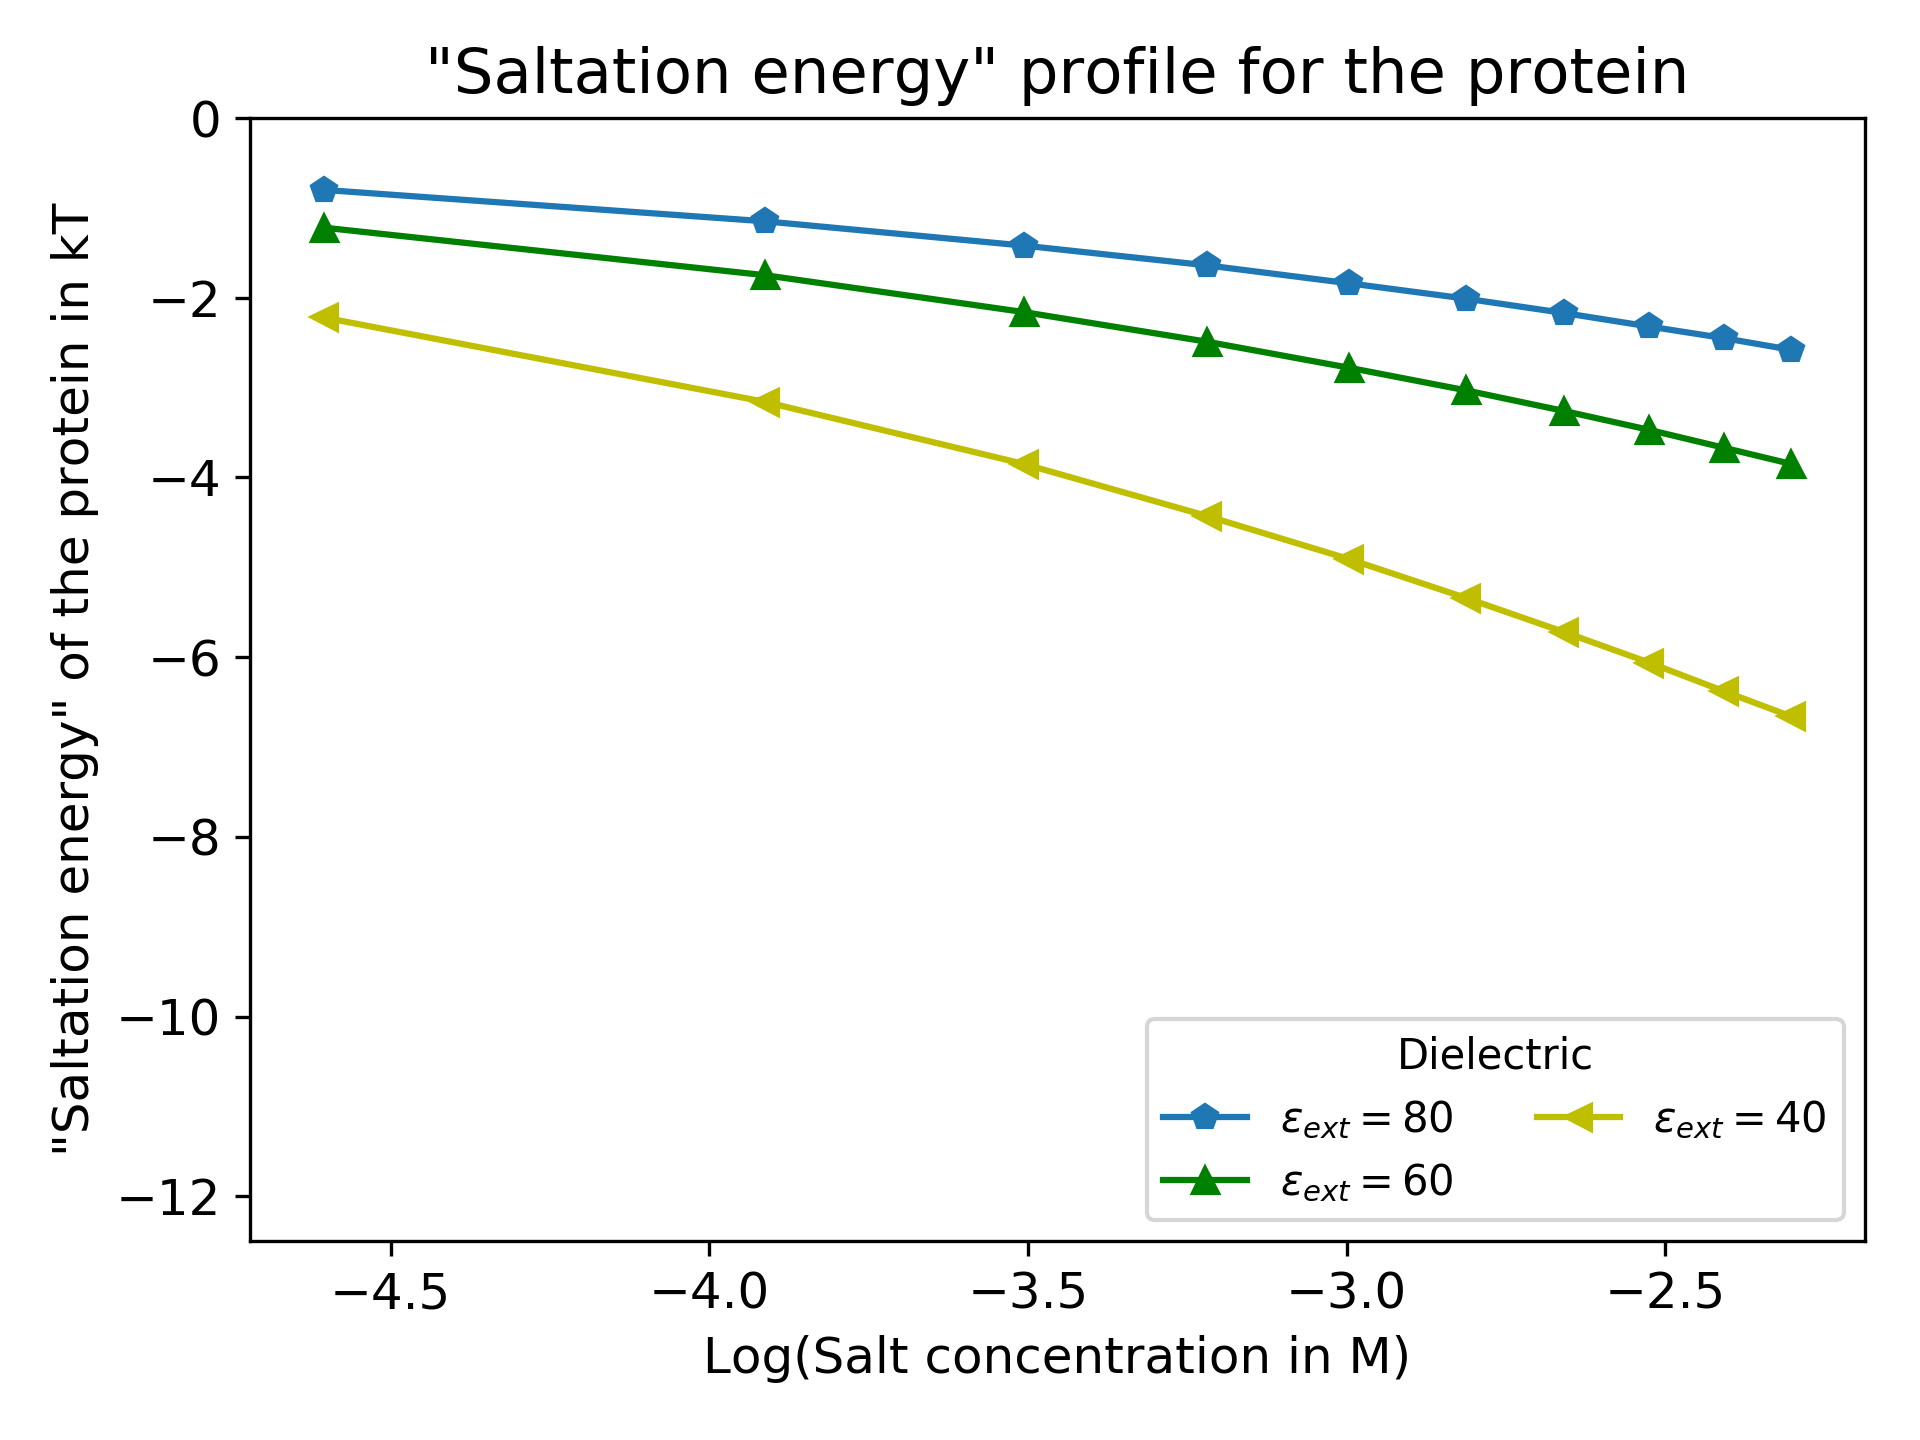
\includegraphics[width=\linewidth]{Figure_8.png}
\caption{The saltation energy computed using DelPhi of the barnase-barstar complex (PDB Id: 1BRS) in different salt concentration and different external dielectric constants.}
\label{fig:plot_saltation_protein}
%% If the optional argument in the square brackets is ``none'', then the caption *will not appear in the main figure at all* and only the full caption will appear under the supplementary figure at the end of the manuscript.
\end{figure}


User may have to define the environment variable \ttvar{$DELPHI_EXE} to match the full path of the DelPhi executable file in the shell. This python script can be executed as below:

\begin{verbatim}
python3 Run-saltation-protein.py
\end{verbatim}

The results of saltation of barnase-barstar complex is shown in Figure \ref{fig:plot_saltation_protein}.

\subsubsection{Computing electrostatic potential on a surface (Zeta potential)} 
DelPhi’s SURFPOT module allows one to obtain the electrostatic potential values on some surface located at some distance from a molecule’s Van der Waals (vdW) surface. The details of its implementation and specific usage can be found in a published work\cite{chakravorty2017new}. A major utility of this kind of calculation is the determination of the zeta($\zeta$)-potential of a molecule or any object for that matter. 

To perform surface potential calculations, a user is required to provide the following lines in the input parameter file:

\begin{verbatim}
SURFPOT=1   !OR SU=1 (0 by default)
SURFDIST=7  !OR SD=7
\end{verbatim}

Parameter \texttt{SURFPOT=1} invokes the \texttt{SURFPOT} module which is not turned on by default. \texttt{SURDIST=7} specifies a distance, in Å, from the solute’s vdW surface where the surface is to be drawn and potentials reported. If \texttt{SURFDIST} is not provided with \texttt{SURFPOT=1} statement, then a default value of 0 is assigned to it. That would mean that the potential on the vdW surface is reported. DelPhi restricts the value of the \texttt{SURFDIST} between 0 and 10Å. It must also be noted that with larger \texttt{SURFDIST} values, the computation time (or DelPhi’s runtime) also increases. 

DelPhi doesn’t print out the surface potential values on the terminal. Instead, it prints out the 3D Cartesian coordinates of the grid-points that constitute the desired surface along with the potentials on it into an ascii-text file. By default, whenever \texttt{SURFPOT=1}, a file called ‘\texttt{sample.zphi}’ is printed. This file will be referred to as a \texttt{zphi} file for the sake of understanding. A user can also alter the name of the \texttt{zphi} file by supplying the following statement in the input parameter file

\begin{verbatim}
OUT(ZPHI, FILE=”_NAME_OF_A_FILE_”)
\end{verbatim}

Along with \texttt{SURFPOT=1} and \texttt{SURFDIST=7} (for example), a zphi format file by the name mentioned via the string replacing \texttt{\_NAME\_OF\_A\_FILE\_} is printed out. A folder with all necessary files is provided as \ttvar{Example_3.1.3/}. 

A \texttt{zphi} format file contains 4 columns – 3 for the x, y and z coordinates of the grid-points (each 10 character long) and 1 for the potential values (15 character long). The units of the coordinates and potential are Å and $ k_BT/e $, respectively. All the lines in the file starting with '\#REMARK' string provide auxiliary information. For example, at the end of the file, DelPhi prints the average value of the potentials on the grid points on that surface as well as the geometric center of the computational box, in the following way:

\begin{verbatim}
#REMARK SIMPLE AVERAGE SURFACE 
                       POTENTIAL = -0.334833 kT/e
#REMARK GEOMETRIC CENTER (ANG)          
                       = 39.335  36.415  34.35
\end{verbatim}

\textit{Visualization of the surface and its potentials}:
The \texttt{zphi} file with the potential and coordinate information can be used for visualizing the surface and the distribution of the potentials on it. It can also be used for other statistical analysis a user might be interested in. To visualize the surface on VMD\cite{humphrey1996vmd}, a TCL script is available for download from \url{http://compbio.clemson.edu/downloadDir/seeSurface.tcl}. The name of the downloaded file \texttt{seeSurface.tcl}

After opening VMD, open its TK Console and type

\begin{verbatim}
% source path/to/seeSurface.tcl
\end{verbatim}

This will load all the functions into the process memory of VMD\cite{humphrey1996vmd}. Then any file, corresponding to a surface can be visualized using the following command on VMD.

\begin{verbatim}
% seeSurface _NAME_OF_ZPHI_FILE_
\end{verbatim}

Replace \texttt{\_NAME\_OF\_ZPHI\_FILE\_} with the path to the \texttt{zphi} file. After the command is executed, it prints information on the console and then draws a surface by drawing the individual points. Each point is assigned a color. The points with the most negative and positive potential value are assigned red and blue colors, respectively. The gradient traverses from the minimum to maximum potential by assigning grid-points red, white and blue colors. An illustration of surfaces, drawn at 3 separate distances around a protein (PDB: 2NVH) is shown in Figure \ref{fig:zeta-potential}. The surfaces are placed at distances of 3, 6 and 9Å from its vdW surface. For better visualization, the protein’s structure is also loaded and represented using the MSMS surface representation. 

\begin{figure*}
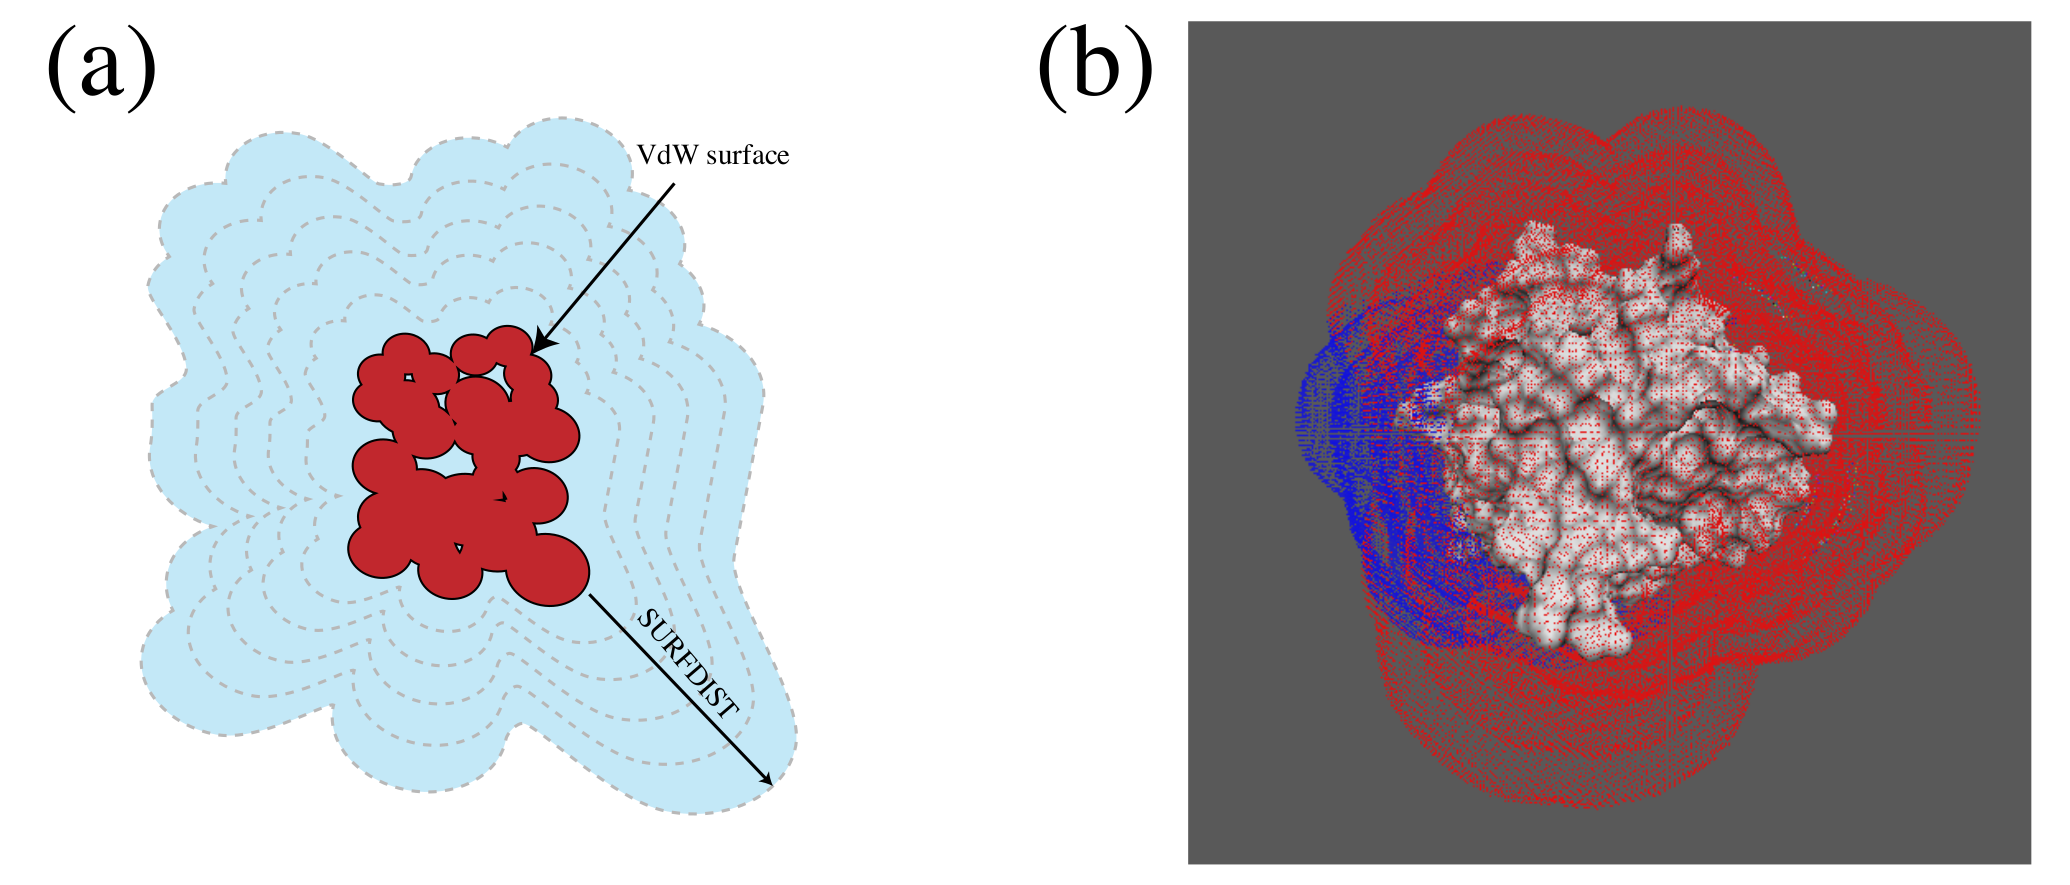
\includegraphics[width=0.95\linewidth]{Figure_9.png}
\caption{SURFPOT module of DelPhi. (a) Schematic showing the placement of surfaces located at increasing distance from the vdW surface of a protein like object (colored in red). (b) An illustration of potential distribution on three distinct surfaces located 3, 6 and 9Å away from the VdW surface of the protein (PDB ID: 2NVH). The red colored grid-points indicate regions with negative potentials and the blue-colored ones indicate regions with positive potentials. The ‘blue’ colored patch on the left shows the small region dominated by positive potentials while the rest of the surface is predominantly positive.}
\label{fig:zeta-potential}
%% If the optional argument in the square brackets is ``none'', then the caption *will not appear in the main figure at all* and only the full caption will appear under the supplementary figure at the end of the manuscript.
\end{figure*}


\subsubsection{Computing electrostatic potential, energy of interaction and forces between two sets of atoms}
In this section, we will describe how to calculate the electrostatic potential, energy of interaction and force between two sets of atoms using ‘\texttt{frc}’ option. Scheme is shown in Figure \ref{fig:elec_force}.

\begin{figure}[hbt!]
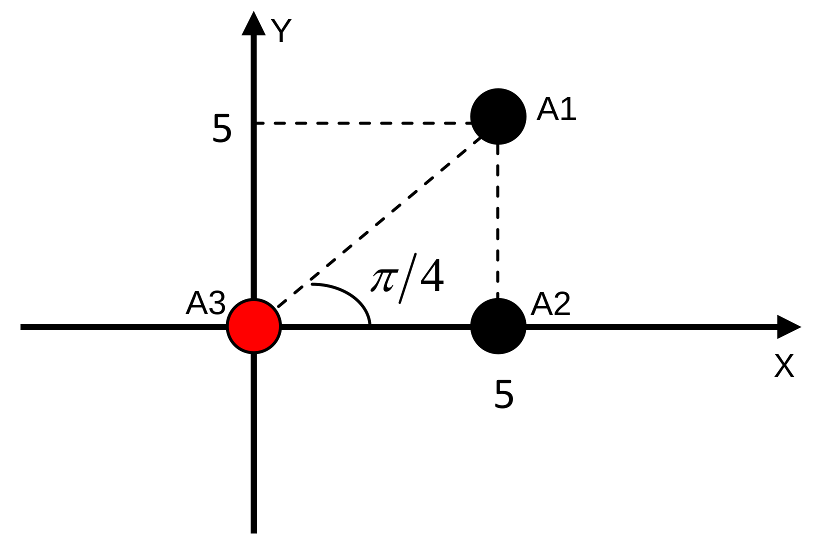
\includegraphics[width=\linewidth]{Figure_10.png}
\caption{The schematic representation of setup of example system for electrostatic potential, energy of interaction and forces between two sets of atoms (A3 due to A1 and A2).}
\label{fig:elec_force}
%% If the optional argument in the square brackets is ``none'', then the caption *will not appear in the main figure at all* and only the full caption will appear under the supplementary figure at the end of the manuscript.
\end{figure}

In the parameter file we need to add command “\texttt{site (argument)}”, specifically in this case \texttt{site(a,p,f)}. This makes DelPhi to report the potentials and electrostatic field components at the positions of the subsets of atoms in the \texttt{frc} file. This calculation needs two sets of \texttt{pdb} files, one is “\texttt{atoms.pdb}” which contains coordinates of all atoms which contribute to the electostaic potential and another is “\texttt{atom-1.pdb}” which contains the dummy atom to specify the coordinate at which the electrostatic potential and electric fields are required to be computed. The charge and size information for all the atoms present in file \ttvar{atoms.pdb} have to be provided in charge and size files \ttvar{atoms.crg} and \ttvar{atoms.siz} respectively. In present case, we attempt to calculate electrostatic potential and electrostatic field at the origin due to a system of two atoms A1 and A2  whose charges are $ q_1 = 10 e_c$ and $ q_2 = 20 e_c $ respectively, the size of both atoms is 1.0 \text{\AA}, and coordinates of A1 and A2 are $ \left(5.0, 5.0, 0.0 \right) $  and $ \left(5.0, 0.0, 0.0\right) $  respectively. Here charges are in unit of charge of a proton i.e. $ e_c $ and distances and coordinates are in \text{\AA}. An schematic representation of the system is  shown in Figure \ref{fig:elec_force}. The analytical expression for such a simplistic system is known (see Eqn. \ref{eqn:frc_at_point}). Therefore, we can benchmark DelPhi results against the analytical value. Since, DelPhi unit of energy is $ \frac{k_BT}{e} $, we shall convert the analytical energy also in $ \frac{k_BT}{e} $ for comparison. Using Boltzmann constant $ k_B = 1.38\times 10^{-23} JK^{-1}$, absolute temperature $ T = 297.33 K $ (default temperature in DelPhi),  elementary charge $ e_c = 1.6 \times 10 ^ {-19} C $, and external dielectric constant $ \epsilon_{ext} = 80 $, the potential computed from Eqn. \ref{eqn:frc_at_point} comes to be 38.035 $ \frac{k_BT}{e_c} $, while potential computed  from DelPhi is 38.1317 $ \frac{k_BT}{e_c} $, which shows a relative error $ \epsilon = \left | \frac{\phi -\phi_{DelPhi}}{\phi} \right | \approx 10^{-3} $ showing an excellent agreement to analytical value. Similarly, analytical values of the X- and Y- components of electric field $ E_x $ and $ E_y $ at position of A3 (see coordinates in \ttvar{atom-1.pdb}) due to  system of charges A1 and A2 are  $ -6.613 \frac{k_BT}{e_c\text{\AA}} $ and $-0.993 \frac{k_BT}{e_c\text{\AA}} $, while values computed from DelPhi are   $ -6.7208 \frac{k_BT}{e_c\text{\AA}} $ and  $ -1.0031 \frac{k_BT}{e_c\text{\AA}} $, respectively, which are also in good agreement to analytical values. All the required files are provided in the directory \ttvar{Example_3.1.4/}

\begin{equation}\label{eqn:frc_at_point}
    \phi = \frac{1}{4\pi\epsilon_0\epsilon_{ext}} \left ( \frac{q_1}{d_1} + \frac{q_2}{d_2} \right)
\end{equation}

We can run DelPhi for this example using command:

\begin{verbatim}
$DELPHI_EXE param_frc.prm > delphi_frc.log
\end{verbatim}

The output \ttvar{frc} file i.e. \ttvar{atoms.frc} contains necessary lines with all the information regarding potential and components of electric field. They can be further used to calculate energy of interaction and force between two atoms. Note that the user can change the grid size and scale according to their need.

\subsubsection{How to do focusing?}

The focusing method is used for computing electrostatic potential and electric field for a molecular system at higher precision by using two or more runs where first run is done with moderate grid resolution for entire molecular system (typically \texttt{scale=1} or \texttt{scale=2}) followed by second run with fine grid resolution (typically \texttt{scale=4}) for only most relevant region of the system.  Thus, the two runs focusing scheme allows to obtain electrostatic potential and electric field with comparable precision to single high grid resolution (\texttt{scale=4}) run incurring comparably lesser computational resources. The schematic representation of focusing is shown in Figure \ref{fig:focusing}. Another advantage of this scheme is that for larger molecular systems high grid resolutions may require very large number of grids hence large memory is needed for computation which may not be available on the computer being used. However, focusing scheme drastically reduces the number of grid points. If the first run is done with scale=1 the memory needed would be \ttvar{~}1/64\textsuperscript{th} of the memory needed for run with \texttt{scale=4}. 

\begin{figure}[hbt!]
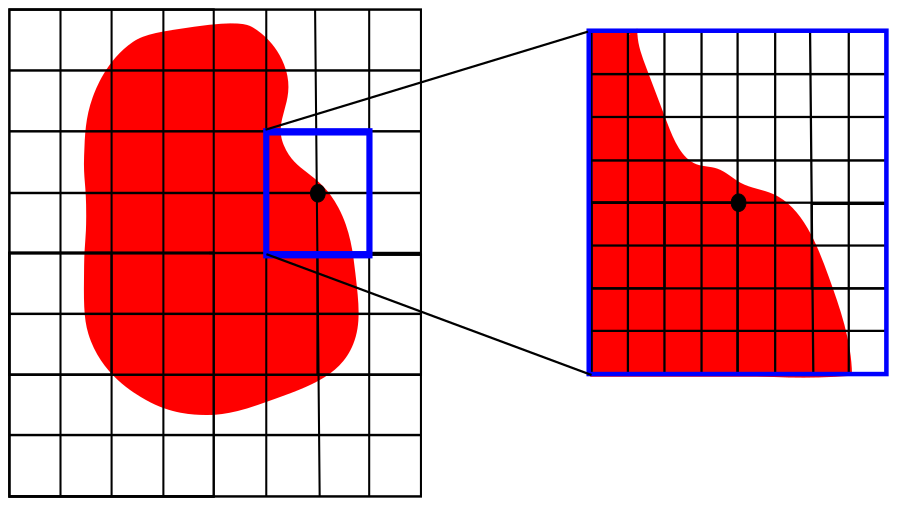
\includegraphics[width=\linewidth]{Figure_11.png}
\caption{A cartoon representation of scheme of focusing run. As shown in left panel the first DelPhi run (parent run) computes the potential and electric force at a lower \texttt{scale=1} for the whole system, followed by the second high \ttvar{scale=4} DelPhi run (child run, shown in right panel). The child run focuses on only region of importance defined by the \ttvar{acenter} marked by black dot, considering only a subset of grids of parent run, but with fine grids, the grid potentials of parent run are used as boundary condition for child run.}
\label{fig:focusing}
%% If the optional argument in the square brackets is ``none'', then the caption *will not appear in the main figure at all* and only the full caption will appear under the supplementary figure at the end of the manuscript.
\end{figure}

The geometric center of the region of interest is used as the focusing center; parameter “\texttt{acenter}” is used for this purpose. Now, we shall explain the process of carrying our focusing run with an example (\ttvar{Example_3.1.5/}) explaining relevant input parameters and outputs to make it more understandable. The example calculates potential and electric field generated by barnase onto a particular residue Asp39 of its partner barstar. We must have following files: 
\texttt{barnase.pdb}, \texttt{amber.crg}, \texttt{amber.siz}, \texttt{barstar-ASP39.pdb}

The first run, less resolution run, is called a parent run. It is executed as:

\begin{verbatim}
$DELPHI_EXE param_phimap1.prm > focusing1.log
\end{verbatim}

This will output \ttvar{phimap1.cube} which is then read by the second “child” run. The acenter to be set to the center of Asp39 of barstar in the child run parameter file. The child run reads the \ttvar{phimap1.cube} and outputs \ttvar{phimap2.cube}. The resolution of the child run is higher than in the parent run (\texttt{scale=4.0}) and the calculation box is smaller; the \texttt{acenter} option is used to indicate where is the center of the child box; the boundary condition is set as 3 to indicate the boundary values are calculated based on the input \texttt{phimap1.cube}; an frc option is used to calculate the potential and field on residue Asp39 of barstar. 
The child run can be done as below.

\begin{verbatim}
$DELPHI_EXE param_phimap2_focus.prm > focusing2.log
\end{verbatim}

The output is written to file named \texttt{frc.out}. The file \texttt{frc.out} provides the electrostatic potential at each atom of Asp39 followed by three columns with the components of the electrostatic field as shown below (data for only the first atom of Asp39 is shown):  

\begin{verbatim}
ATOM DESCRIPTOR  GRID PT.   GRID FIELDS: (Ex, Ey, Ez)  
N    ASP   39    4.1756   0.6405   -0.3778   -0.3490
total energy = -3.39614 kt
\end{verbatim}


\subsubsection{Electrostatic component of binding energy} \label{sec:elec_binding}
To demonstrate how to use DelPhi for computing electrostatic component of protein-protein binding we have taken barnase-barstar as the system. First we are required to prepare the coordinate, charge, size and parameter files for each of the three cases: barnase-barstar complex, barnase and barstar. The required files are provided in directory \ttvar{Example_3.1.6/}. This folder should have the following five files (\ttvar{barnase-barstar.pdb}, \ttvar{barnase.pdb}, \ttvar{barstar.pdb}, \ttvar{c22.crg} and \ttvar{c22.siz}) and two directories (\ttvar{2-dielectric/} and \ttvar{gaussian/}). The \ttvar{.pdb} and \ttvar{.crg} files contain the coordinate information and partial charge of the all atoms respectively for the barnase-barstar, barnase and barstar systems. In the present example we will use partial atomic charges and atomic Van der Waals radii from provided \ttvar{c22.crg} and \ttvar{c22.siz} files respectively. 

\begin{figure*}
\centering{
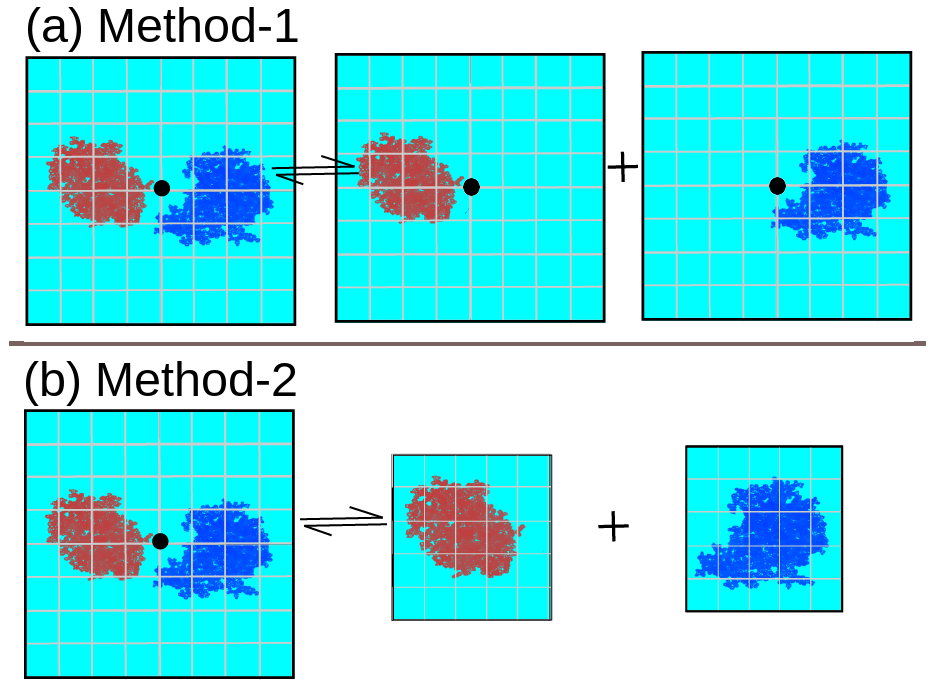
\includegraphics[width=0.75\linewidth]{Figure_12.png}
}
\caption{Two methods for computing the electrostatic component of binding free energy. The black dot in Figure represents the \texttt{acenter} for DelPhi runs. Note that in panel (a) bound and unbound molecules are positioned at the same place in the same grid, while in panel (b) bound and unbound molecules are not.}
\label{fig:elec_comp_bind_energy}
%% If the optional argument in the square brackets is ``none'', then the caption *will not appear in the main figure at all* and only the full caption will appear under the supplementary figure at the end of the manuscript.
\end{figure*}

\textbf{Electrostatic component of binding energy using traditional two-dielectric approach}.
The electrostatic component of binding energy can be obtained by two methods, Method-1 uses difference in grid energies, and Method-2 uses energy partitioning. In this process, three DelPhi runs are required as follows; the first run will be on the complex, second on the barnase and the third on the barstar molecules. One should keep the molecules at the same positions in all runs (this is mandatory for Method 1 calculations, since it uses grid energy differences and artificial grid energy terms must be canceled out). The scheme for two method is shown in Figure \ref{fig:elec_comp_bind_energy}.
The files used in this example are present in \ttvar{Example_3.1.6/} and \ttvar{Example_3.1.6/2-dielectric/} directories, change current working directory to \ttvar{Example_3.1.6/2-dielectric/}. Now we can do the DelPhi run using following command.

\begin{verbatim}
$DELPHI_EXE param_barnase-barstar_2-diel.prm \
    > param_barnase-barstar_2-diel.log
$DELPHI_EXE param_barnase_2-diel.prm \
    > param_barnase_2-diel.log
$DELPHI_EXE param_barstar_2-diel.prm \
    > param_barstar_2-diel.log
\end{verbatim}

The energy details for each of three runs is written in \ttvar{barnase-barstar_2-diel.dat}, \ttvar{barnase_2-diel.dat} and \ttvar{barstar_2-diel.dat} files respectively. The relevant contents of the three \ttvar{.dat} files are as below.
\begin{verbatim}
The content of barnase-barstar_2-diel.dat
Total grid energy               : 132916.29 kT
Corrected reaction field energy :  -1737.31 kT
Total coulombic energy          : -44990.50 kT
Total required energy (
everything calculated but grid) : -46727.80 kT
\end{verbatim}
\begin{verbatim}
The content of barnase_2-diel.dat
Total grid energy               :  73515.44 kT
Corrected reaction field energy :  -1020.38 kT
Total coulombic energy          : -25009.84 kT
Total required energy (
everything calculated but grid) : -26030.23 kT
\end{verbatim}
\begin{verbatim}
The content of barstar_2-diel.dat
Total grid energy               :  59388.54 kT
Corrected reaction field energy :   -1265.7 kT
Total coulombic energy          : -19433.73 kT
Total required energy (
everything calculated but grid) : -20699.43 kT
\end{verbatim}

Now the electrostatic component of binding energy using Method-1 can be obtained from total grid energies of barnase-barstar complex, barnase and barstar as follows:
\begin{equation}
\begin{aligned}
\Delta G(bind) &= G_{grid}(cpx) - G_{grid}(barnase) - G_{grid}(barstar) \nonumber \\
\Delta G(bind) &= 132916.29 - (73515.44 + 59388.54) kT \nonumber \\
&= 12.31 kT \nonumber \\
\end{aligned}
\end{equation}

The electrostatic component of binding energy using Method-2 can be obtained from partitioned energies as follows
\begin{equation}
\begin{aligned}
\Delta G(bind) &= G_{Coulombic} + G_{\text{reaction field}} + G_{ions}\\
               &= G_{ARET}(complex) - G_{ARET}(barnase) - G_{ARET}(barstar) \\
               &= -46727.80 - (-26030.23 + -20699.43) kT \\
               &= 1.86 kT \\
\text{where ARET} &= \text{all required energy terms} \\
\end{aligned}
\end{equation}            
Note that the calculated electrostatic component of binding energy via Method-1 and Method-2 is different. This is due to the fact that Method-1 does not fully cancel so termed ``artificial grid energy'' arising from real charges partitioning onto the grid. Thus, we recommend using Method-2, the energy partitioning method in case of energy calculations with zero salt. The reason is that current version of DelPhi does not support the option of explicit calculations of the energy of interactions between mobile ions and permanent charges (see \cite{rocchia2001extending} for more details).

\textbf{Electrostatic component of binding energy Gaussian approach}.
In the Gaussian approach there is no strict solvent-solute boundary which separates the mediums of two different dielectric, rather the regions in solute and solvent are described with smooth dielectric function. Because of this fact, energy partitioning described in previous paragraph is not applicable. Therefore, the grid energy of the system which implicitly accounts Coulombic and polar component of the solvation energy is used in this case. However, to be able to obtain electrostatic component of binding, we must use the same point as grid center and same number of grid sizes and scale for complex and monomers. To keep the same point as grid center, one can compute the center of complex and use \ttvar{acenter} input command as \texttt{acenter(xc, yc, zc)} (where \ttvar{xc}, \ttvar{yc}, \ttvar{zc} are the x, y, z coordinates of center for the complex) in all the three calculations. In addition, we are required to activate the Gaussian module by providing \texttt{gaussian=1} in the parameter and the \texttt{sigma=0.65} parameter for the gaussian.
We can add the following set of parameters and their respective values to the parameter files for Gaussian run using Delphi for present example.
\begin{verbatim}
acent(28.459,36.960,8.674)
gaussian=1
sigma=0.65
srfcut=20
\end{verbatim}
\ttvar{Example_3.1.6/} and \ttvar{Example_3.1.6/gaussian/} directories, change current working directory to \ttvar{Example_3.1.6/gaussian/}. Now we can do the Delphi run using following command.
\begin{verbatim}
$DELPHI_EXE param_barnase-barstar_gauss.prm \
                   > param_barnase-barstar_gauss.log
$DELPHI_EXE param_barnase_gauss.prm \
                   > param_barnase_gauss.log
$DELPHI_EXE param_barstar_gauss.prm \
                   > param_barstar_gauss.log
\end{verbatim}
The total grid energies for barnase-barstar complex, barnase and barstar are found from the respective .dat files and the electrostatic component of binding is computed as below via Method-1. 15975.45 - (8825.55 + 7165.57) kT = -15.67 kT. In the present case, note that the electrostatic component of binding energy is very different from the energy calculated with traditional two-dielectric approach. This is due to different dielectric distribution applied in these two approaches. One should use the traditional two-dielectric if modeling involves rigid structures (energy minimized or snapshots from MD simulations). The Gaussian approach is applicable for cases when one wants to use single structure to generate ensemble average quantity (see \cite{chakravorty2018gaussian} for more details).


\subsubsection{Salt dependence of binding energy using traditional two-dielectric model}
Charges of salt ions introduce extra sources of electric fields and affect the electrostatic interactions between the molecules. This example is designed to capture this salt dependence of binding energy using traditional two-dielectric model. The required files for this example are provided in folders \ttvar{Example_3.1.7/} and \ttvar{Example_3.1.7/saltation/}. The electrostatic component of binding energy using traditional two-dielectric approach via difference of grid energies  is used. In order to calculate the salt dependence of binding energy we are needed to compute binding energy twice, once at zero salt concentration and second time at desired non-zero salt concentration. The difference of binding energy between non-zero salt case and zero-salt case is the required salt dependence of the binding energy at given salt concentration. However, to find out the relationship between the change in binding energy due to varying salt concentration, here binding energy is calculated at multiple salt concentrations starting from 0.02M to 0.2M in steps of 0.02M and difference from zero-salt binding energy is recorded. The salt dependence of binding energy is plotted against the logarithm of the salt concentration, in addition the linear fit in the two quantities are also performed and coefficients of fit are reported in Figure \ref{fig:plot_saltation_pp_binding}.

\begin{figure}[hbt!]
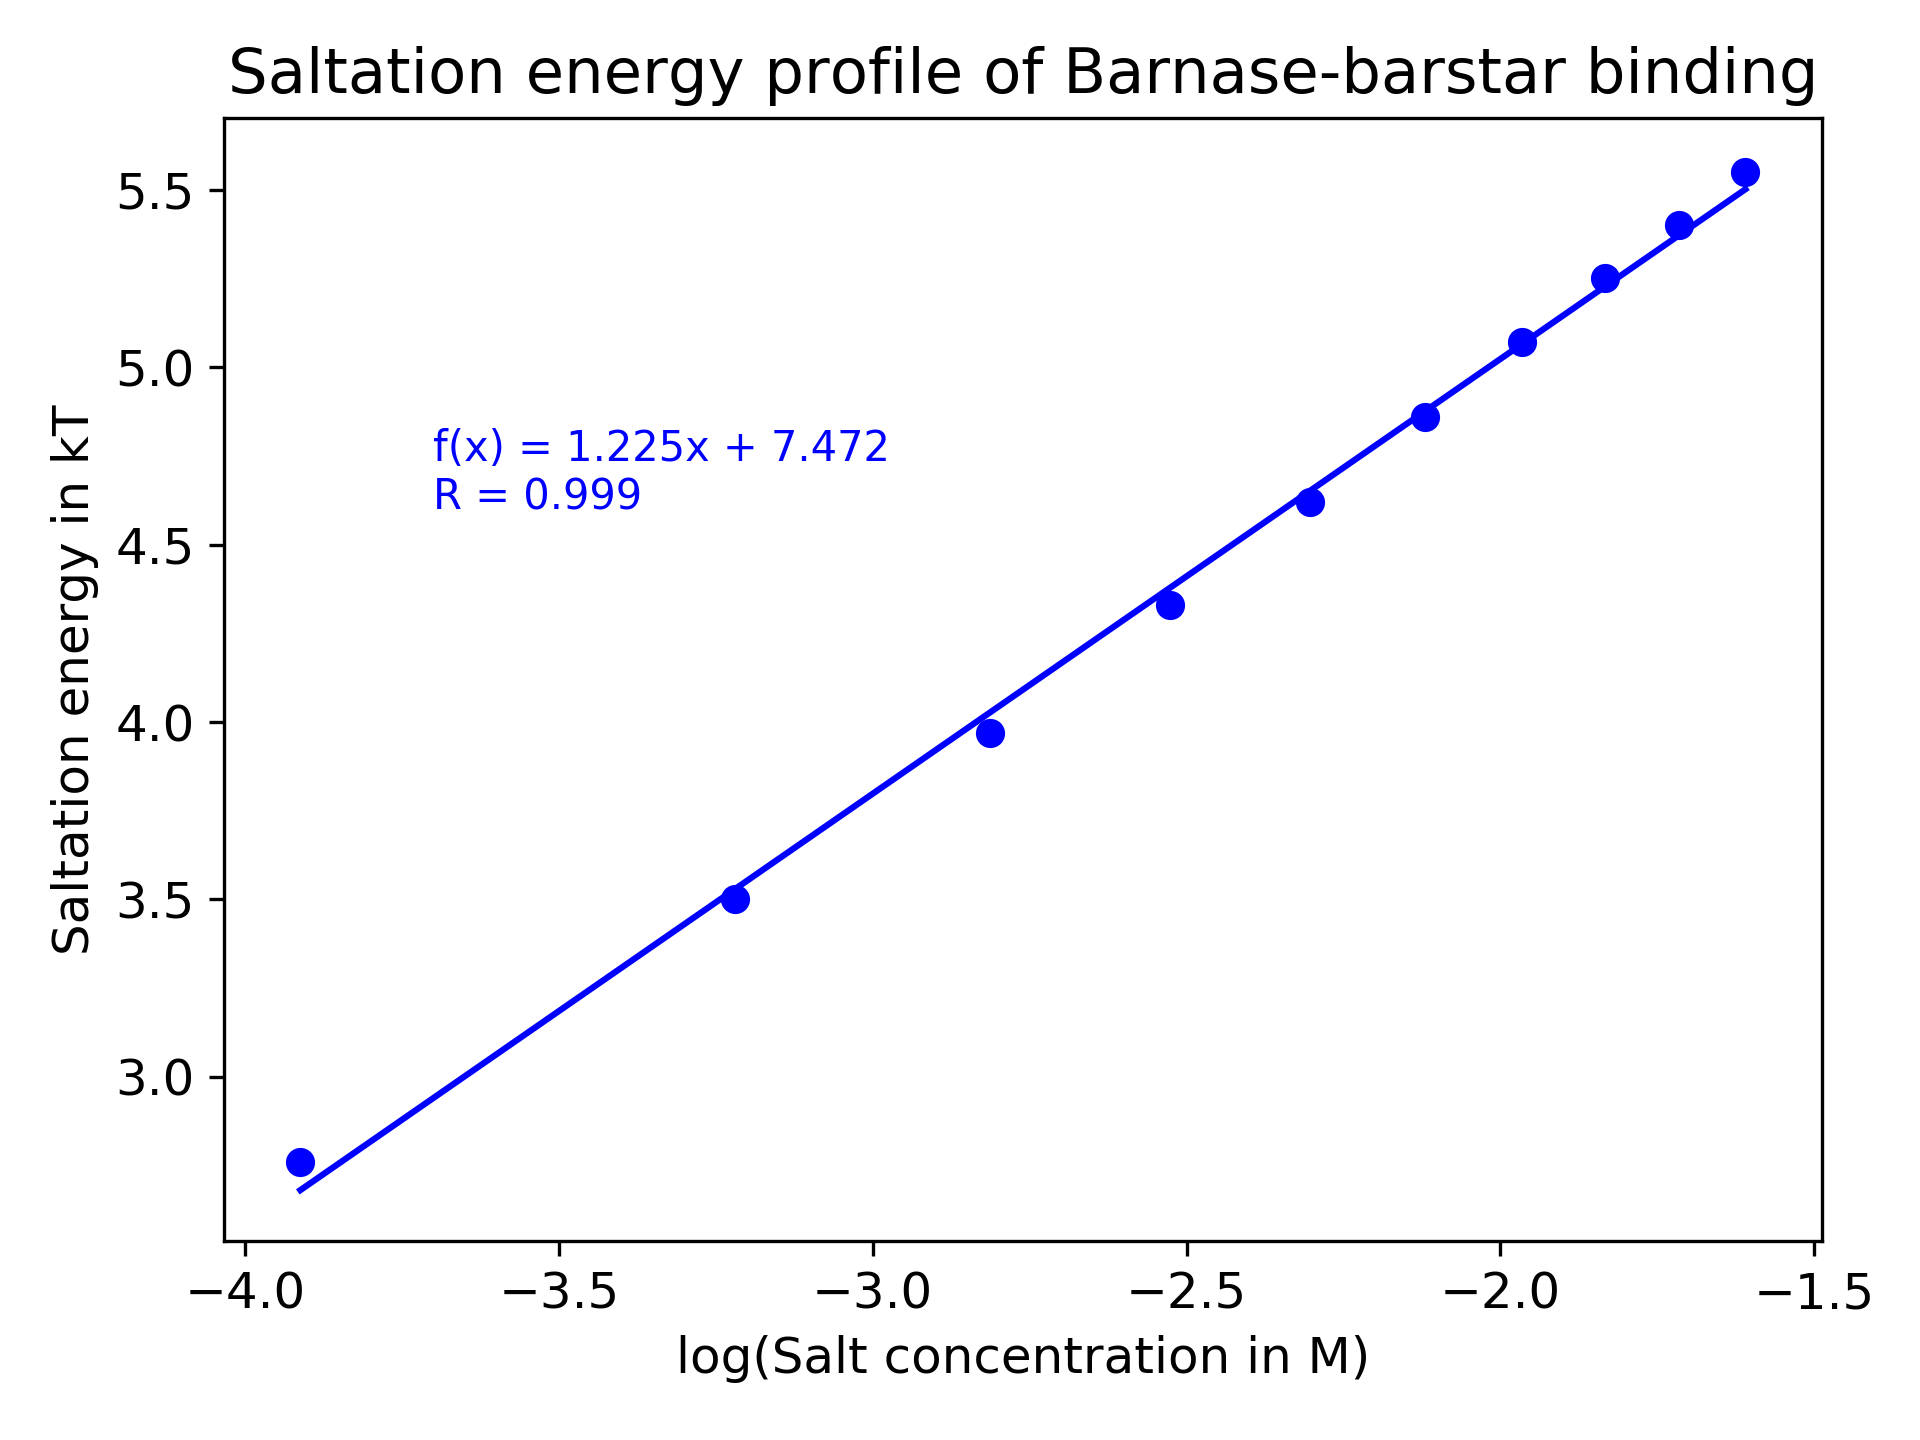
\includegraphics[width=\linewidth]{Figure_13.png}
\caption{The salt dependence of binding energy of barnase-barstar using two-dielectric approach implemented in DelPhi.}
\label{fig:plot_saltation_pp_binding}
%% If the optional argument in the square brackets is ``none'', then the caption *will not appear in the main figure at all* and only the full caption will appear under the supplementary figure at the end of the manuscript.
\end{figure}

Performing these calculations requires three different DelPhi runs for each binding case and there are 11 such cases (1 zero-salt and 10 non-zero salts varying from 0.02 M to 0.2 M in steps of 0.02 M), requiring total 33 DelPhi runs. Therefore, to facilitate running these DelPhi calculations a bash script \texttt{RUN\_DELPHI\_SALTATION.sh} is provided in the directory \texttt{Example\_3.1.7/saltation/}. This script creates parameter files for DelPhi, runs DelPhi and stores log files on the fly. In addition, the bash script also parses relevant energy outputs from the log files for each run to compute salt dependence of binding energy and saves these results in file \ttvar{saltation_using_M1_for_biniding.dat}. However, if environment variable \ttvar{DELPHI_EXE} is already not set then users are needed to set the absolute path of DelPhi executable file in the environment variable \ttvar{DELPHI_EXE} before running it as below:

\begin{verbatim}
bash RUN_DELPHI_SALTATION.sh
\end{verbatim}

After successfully running the bash script, the plot can be generated by running python script \texttt{plot-saltation.py} as:

\begin{verbatim}
python3 plot-saltation.py
\end{verbatim}

            
\subsubsection{Salt dependence of the binding energy using Gaussian model}
As mentioned above charges of salt ions introduce extra sources of electric field and affect the electrostatic interactions between the molecules.  Take the example of the protein-protein complex, `COLICIN E9 DNAse Domain with its Cognate Immunity Protein Im9' (PDB ID: 1EMV) involving the interaction of two helical (all-$ \alpha $) chains, A and B. The salt dependence of binding free energy can be given by the change of binding free energy under variance of salt concentrations in the solvent. Step one, the ‘total grid energy’ is to be computed for both the free chains (A, B) as well as the complex (AB), two times; first, at `zero' salt and then at another salt concentration, e.g. physiological salt (0.15 M). Let these terms be $ \Delta G_{nz_{AB}}$, $ \Delta G_{nz_A}$, $ \Delta G_{nz_B}$ (for AB, A and B chains at non-zero salt), $ \Delta G_{z_{AB}}$, $ \Delta G_{z_A} $, and $ \Delta G_{z_B}$ (at zero salt). From these terms, the de-saltation energy component is:
\begin{equation}
 \Delta\Delta G_{saltation}= \Delta\Delta G_{salt_{AB}}  - \left( \Delta\Delta G_{salt_A}  + \Delta\Delta G_{salt_B} \right)
\end{equation}
where,
\begin{equation}
\begin{aligned}
\Delta\Delta G_{salt_{AB}}  &= \Delta G_{nz_{AB}}  - \Delta G_{z_{AB}}
\nonumber \\
\Delta\Delta G_{salt_A}  &= \Delta\Delta G_{nz_A}  - \Delta\Delta G_{z_A} \nonumber \\
\Delta\Delta G_{salt_B}  &= \Delta\Delta G_{nz_B}  - \Delta\Delta G_{z_B} \nonumber
\end{aligned}
\end{equation}
The salt dependence of binding free energy can be calculated under Gaussian smooth boundary by involving \texttt{gaussian=1}\cite{jia2017treating}. 

Each calculation of the binding free energy under given salt concentration is the same as the calculation of electrostatic component of binding free energy (see \ref{sec:elec_binding}). After multiple repeats of the calculation under different salt concentration, the change of binding free energy over salt concentration is the salt dependence of binding free energy.

In the \texttt{Example\_3.1.8}, the salt dependence is calculated using binding free energy under two different salt concentrations, 0 and 0.15M. Usage of grid energy is recommended when calculating salt dependence. One can do DelPhi calculations at varying salt concentration by executing the provided bash script \ttvar{run.sh} as given below:

\begin{verbatim}
bash run.sh
\end{verbatim}

The output from DelPhi should be as following,

\begin{verbatim}
Salt: 0M 
 Energy> Total grid energy : 63971.15 kT
 Energy> Total grid energy : 24138.68 kT
 Energy> Total grid energy : 39785.12 kT
\end{verbatim}

\begin{verbatim}
Salt: 0.15M
 Energy> Total grid energy : 62767.11 kT
 Energy> Total grid energy : 23693.72 kT
 Energy> Total grid energy : 39008.93 kT
\end{verbatim}

\begin{equation}
\begin{aligned}
\Delta \Delta G_{salt_{complex}} - (\Delta G_{nz_{complex}} + \Delta G_{z_{complex}}) &: -1204.04 \nonumber \\
\Delta\Delta G_{salt_{mol1}} - (\Delta G_{nz_{mol1}} + \Delta G_{z_{mol1}}) &: -444.961 \nonumber \\
\Delta\Delta G_{salt_{mol2}} - (\Delta G_{nz_{mol2}} + \Delta G_{z_{mol2}}) &: -776.19 \nonumber \\
\Delta\Delta G_{saltation} &: 17.11 \nonumber 
\end{aligned}
\end{equation}

\subsubsection{Non-linear PBE's applications for electrostatic binding energy of peptide to membrane}
When the system of interest is highly charged, the non-linear effects may be significant and should be taken into consideration via solving non-linear PBE (NLPBE). This is illustrated in \texttt{Example\_3.1.9}, where the electrostatic binding energy is calculated in case of peptide at distance 4 \text{\AA} from a lipid membrane. One computes the total non-linear grid energy for the complex ($ \Delta G_{cplx}$), the membrane ($ \Delta G_{mbrn}$) and peptide ($ \Delta G_{pept} $), keeping their positions the same and using the same "scale" value. Then one subtracts these energies as shown in Eqn. \ref{eqn:deldelg_nlpbe}.
\begin{equation}\label{eqn:deldelg_nlpbe}
\Delta\Delta G_{binding}(d) = \Delta G_{cplx}(d) - \Delta G_{mbrn}(d) - \Delta G_{pept}(d)
\end{equation}

at the corresponding distance ``$ d = 4 \text{\AA} $'' and obtains the electrostaic component of binding energy $ \Delta\Delta G_{binding}(d) $. The requirement for keeping the complex, the membrane and the peptide at the same position and same scale is to cancel the artificial grid energy.

The DelPhi run for the present example case can be done by executing the command in the example directory \texttt{Example\_3.1.9} as below:
\begin{verbatim}
bash binding.sh
\end{verbatim} 

The script will execute 12 DelPhi runs, each set of 4 runs will calculate the energy of 5-lys, membrane itself and the complex. In order to improve the resolution computation efficient focusing scheme is used for solving non-linear Poisson-Boltzmann equation (NLPBE). Note that in present case, simplified charges are used for lipids, so some of the atoms do not have partial charges.

The total non-linear grid energies for complex ($ \Delta G_{cplx}(4 \text{\AA}) $), membrane ($ \Delta G_{mbrn}(4 \text{\AA}) $) and peptide ($ \Delta G_{pept}(4 \text{\AA}) $) can be obtained from log files \texttt{lys5\_r4\_2.log}, \texttt{r4\_2.log} and \texttt{lys5\_2.log} respectively. These values are 285679.17 kT, 283099.28 kT and 2587.42 kT respectively. Thus, the binding energy $\Delta\Delta G_{binding}(4 \text{\AA}) $ is:

\begin{verbatim}
(285679.17 -2587.42 -283099.28) kT = -7.53 kT
\end{verbatim}

Note that in case of NLPBE, the electrostatic energy has two additional components, namely electrostatic stress and osmotic pressure. Such energy partitioning was originally developed by Kim Sharp \cite{sharp1990calculating}.

\subsection{Set of tutorials for DelPhi associated resources}

\subsubsection{DelPhi Force}

DelPhiForce\cite{li2017delphiforce} is developed and made available within DelPhi distribution to calculate electric field, forces, and energy for a two-molecule system. It can be downloaded from the DelPhi webpage at \url{http:// compbio.clemson.edu/downloadDir/delphiforce.tar.gz}. The DelPhiForce web server is available at \url{http://compbio.clemson.edu/delphi-force/}. Using DelPhiForce output files, the electrostatic forces can be visualized in VMD\cite{humphrey1996vmd}. Once \texttt{DelPhiForce.tar.gz} is downloaded. In the \texttt{DelPhiForce/bin} folder, there are several files e.g. 
\texttt{DelPhiForrce.sh}, \texttt{ForceGen.sh}, \texttt{draw\_arrow.tcl} which will be used in this example.

The two input files required to run DelPhiForce are reference molecule (\ttvar{file1}) and probe molecule (\ttvar{file2}), both of which are in \texttt{.pqr} format. To run the DelPhiForce, go to the example folder, copy all files from the DelPhiForce/bin/ folder to it, then run DelPhiForce using command below:

\begin{verbatim}
./DelPhiForce.sh -1 file1 -2 file2 \
    -e absolute_path_to/delphicpp -o out
\end{verbatim}

After the run, you will get following output files:

\texttt{out.residue}: It is the result of the electrostatic forces on all residues of probe molecule.

\texttt{out.atom}: It is the result of the electrostatic forces on all the atoms of probe molecule.

\texttt{out\_residue.tcl}: It is generated for the visualization of electrostatic force on all residues of probe molecule in VMD\cite{humphrey1996vmd}.

\texttt{out.tcl}: It is generated for the visualization of the total electrostatic force of the probe molecule in VMD\cite{humphrey1996vmd}.

In order to visualize the forces, first launch VMD, open \ttvar{file2}. Then, in the VMD Tk Console, run the commands: 

\begin{verbatim}
source draw_arrow.tcl
source out_residue.tcl
source out.tcl
\end{verbatim}

Then open the \ttvar{file1} in VMD. The electrostatic force will be displayed.  Each arrow illustrates an electrostatic force on a residue of probe molecule. The tail of an arrow is the mass center of the corresponding residue. 

\begin{figure}[hbt!]
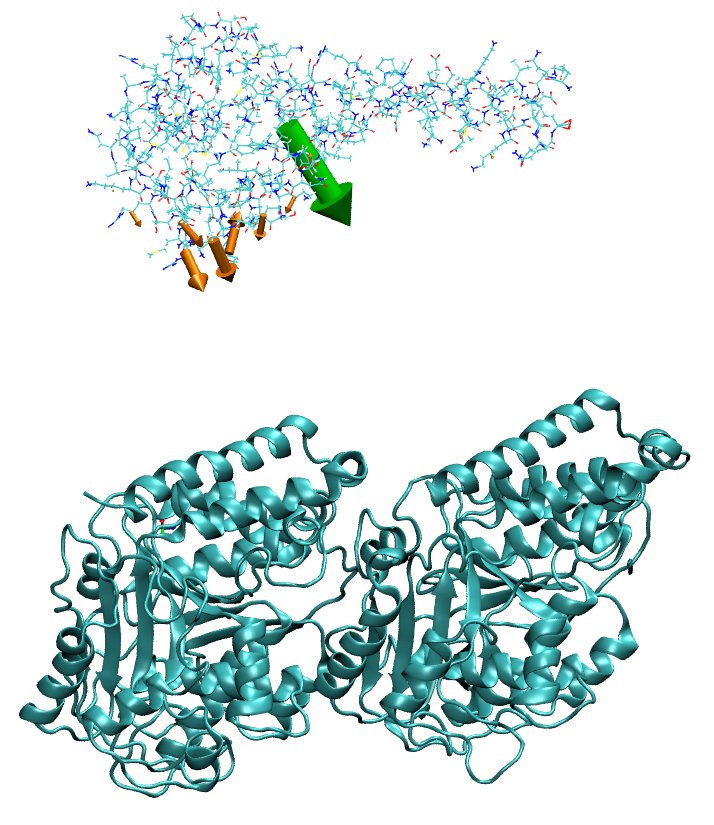
\includegraphics[width=\linewidth]{Figure_14.png}
\caption{Electrostatic forces generated by tubulin dimer (cyan colored cartoon representation) on to kinesin microtubule binding domain (line representation), placed 15 $\text{\AA}$ away from its bound position. Orange arrows represent forces acting on each residue, while the green arrow shows total resultant force. The length of arrow reflects the calculated magnitude of the force.}
\label{fig:delphiforce}
\end{figure}

\subsubsection{DelPhi Force Molecular Dynamics (DFMD)}

The DFMD method\cite{peng2019DFMD} combines accurate long-range electrostatic force calculations via DelPhiForce with a major molecular dynamics simulation package NAMD\cite{phillips2005scalable}.  As a result, the DFMD delivers correct electrostatic forces and applies them in the MD simulations resulting in fast and accurate binding protocol. Typical implementation of Generalized Born (GB)\cite{onufriev2000modification} model in MD involves cut-offs, for both the calculations of Born radii and pair-wise energies. Removing the cut-offs makes MD simulations very slow. However, if the cut-offs are applied, the GB calculated energies are incorrect in case of receptor-ligand separated by large distance, which motivated us to use DelPhiForce to calculate corresponding electrostatic forces and promoted development of DFMD. It can be downloaded from \url{http://compbio.clemson.edu/downloads}

In DFMD, ligand is placed at a distance away from the receptor assuring that long-range electrostatic force are dominating the driving of binding. Then the electrostatic forces acting on the each atom of the ligand by the receptor are computed with DelPhiForce\cite{li2017delphiforce}. The forces are given to steered MD module of NAMD and then short steered MD simulation is carried out. A new position and orientation after the shot simulation are subjected to DelPhiForce to update the atomic forces and iterations are then repeated for another cycle.

Files needed in user’s directory:
Input pdb files for receptor, Input pdb files for target, and Amber prepi and frcmod files for ligands: These files are topology files for MD simulation of ligand and can be generated by antechamber in Amber tools. These files should be put in SOURCE/parameters. The \texttt{DelhiForce\_MD.py} also needed to read the MD parameters files in SOURCE folder. If the path to the SOURCE folder is changed, the new path should be specified using original arguments \texttt{–p}.

Parameters of DFMD simulations:
\begin{enumerate}
\item Number of steps for each cycle to update the steered force: In DFMD, the MD simulation cycle is set to 500 steps, which generally results in good performance and reasonable computing time based on our benchmarking using the Spermine Synthase systems. Users are given the option to adjust this parameter in their simulations.

\item Steered electrostatic force range ($ F_{lower} $, $ F_{upper} $): When the target is away from the receptor, the computed electrostatic forces can be too small to be read by NAMD. Upon the ligand getting contact with proteins, the computed electrostatic forces can be large (for example tens of kcal/mol/Å). Thus, we provide user to set up minimal force and maximum force ($ F_{lower} $, $ F_{upper}$) to avoid large unfavorable artificial effects in the simulation.

\item Cycle number: The number of DelPhiForce calculations and updating cycles in the simulation.

\item Cut off distance: The cut-off distance used in GBIS MD.

\item Diffusion constant of the simulation: In the simulation, Langevin dynamics is applied for the modeling of dynamics of the molecular system, where the diffusion effects are simulated via randomly applied forces and velocity dependent frictions. We provide users with an option to adjust the damping coefficient if needed.

\item Simulation mode: Based on type of simulation users are provided with three different simulation modes: Accelerated mode, such that the atomic DefPhiForce are calculated constantly until the end of the simulation; Cut-off mode, such that the atomic DelPhiForces are calculated only for ligand atoms far away from the receptor than the cut-off distance in MD simulations ; Scaled mode, such that the atomic DelPhiForces are corrected for force calculated via GB, which guarantees that there is no double counting of electrostatic force in MD.

\item Path to the parameter files: Path to the NAMD and DelPhi Executable files and MD parameter files are required. These files are originally in SOURCE folder. If the path to the SOURCE folder changed, new path should be provided.

\item Path to VMD: DFMD require VMD for trajectory analysis, so path to the executable VMD should be provided.
\item 
Procedures to run the simulations:
\begin{enumerate}
\item The DFMD are recommended to be run on the cluster.  In the folder with all prepared input files, the following command is used to start the simulation:

\begin{verbatim}
python DelphiForce_MD.py \
-l SCALE_LOW(default = 0.2 kcal/mol/Å) \
-u SCALE_UP(default = 1.18 kcal/mol/Å) \
-n CYCLE_NUMBER(default = 8000) \
-f FORCE_UPDATING_FREQUENCY(default = 500) \
-c CUT_OFF(default = 18 Å) \
-d LANGEVIN_DAMPING(default = 1) \
-m 10 \
--simulation_mode {1,2,3} (default = 1) \
-p PATH_TO_PARAMETERS_FILES \
-v PATH_TO_VMD \
receptor_PDB \
target_PDB
\end{verbatim}

\item During the running of the simulations, all the steered MD output raw files are in the out folder. For the convenience of visualization and analysis of the trajectory, the short trajectories of each short cycle are automatically concatenated and the concatenated DCD files of the entire simulation are provided in \texttt{./DCD/combine.dcd}.
\item VMD is recommended to analyze the DCD files. To visualize the simulation trajectories, type the command:

\texttt{mol load complex.prmtop dcd ./DCD/combine.dcd}

in the TCL interface of the VMD. Users are also recommend to compute the RMSD of target in respect to the binding site for quantitative analysis.
\end{enumerate}
\end{enumerate}

\subsubsection{SAAMBE}
The Single Amino Acid Mutation based change in Binding free Energy (SAAMBE)\cite{petukh2015predicting} web-server predicts the change of protein binding free energy due to a mutation. The web-server\cite{petukh2015predicting,petukh2016saambe} can be accessed via \url{http://compbio.clemson.edu/saambe_webserver/}. 
The user input section is categorized into three sections:
\begin{enumerate}
    \item PDB selection: In this section, user need to provide a structure file by uploading a PDB file from their local file system.
    
    \item Partner selection: There are two inputs (Partner 1 and Partner 2) in this section. User must supply the chain of partner 1 and chain of partner 2 respectively as the input. If multiple chains construct partner 1 or partner 2, user needs to provide all the chains. For example, if chain A and chain B construct partner 1, then user must provide AB in place of Partner 1.
    
    \item Mutation: This section contains four sub sections:
    \begin{enumerate}
	    \item Position: position of the particular residue, i.e. the residue number, which is replaced in the mutant, need to be provided in the box.
	    
	    \item Chain: chain ID at which mutation occurs.
	    
	    \item Original amino acid: amino acid type in wild type protein.
	    
	    \item Mutated amino acid: amino acid type in mutant protein.
    \end{enumerate}
\end{enumerate}
Once the user submits the job, it is directed to a different page and the job status is displayed as ``Your job is still running and will come back later''. If all the correct information is supplied, after the job finishes successfully, the result page displays “Job Status: Your job run successfully”. Following three downloadable output result files are generated and user can click the link to download them.

\textit{ Result File}: The file has the information of change in binding free energy due to mutation along with the change of the various contributing energy components.

\textit{Download WT Structure}: Energy minimized 3D structure of wild type protein.

\textit{Download MT Structure}: Energy minimized 3D structure of mutated protein.

If the job fails, an error txt file is generated as output, which provides the information about the job failure. The web page keeps on informing the user when the job is created, when it starts and if it’s still running.

The front page of SAAMBE provides a link to download a PDB file (1BRS.pdb), to be used for training purposes. The link guides the user how to use the file, and what are expected results. In summary, if one submits PDB file (1BRS.pdb) and request residue GLU at position 80 of chain D to be mutated to ALA, the SAAMBE predicts that this mutation will de-stabilize the complex by $ \Delta\Delta G_{pred} =$ 0.46708 kcal/mol. The corresponding experimentally determined $ \Delta\Delta G_{exp} $ is  0.48415 kcal/mol, which is very close to predicted.

\subsubsection{SAMPDI web-server}
Protein–DNA interactions are essential for many important cellular processes and mutations occurring in DNA-binding protein have profound effect on protein-DNA interactions. This is the reason why many diseases are caused by the change of native binding energy. SAMPDI\cite{peng2017predicting} Web Server provides fast and accurate predictions for the effects of single amino acid substitution on the binding free energy of protein-DNA complex. This method utilizes modified molecular mechanics Poisson-Boltzmann Surface Area (MM/PBSA) approach along with an additional set of knowledge-based terms delivered from investigation of the physico-chemical properties of protein-DNA complexes. Important feature is applying DelPhi Gaussian-based smooth dielectric function to calculate the change of solvation energy. The method is implemented in a web-server (\url{http://compbio.clemson.edu/SAMPDI/}), which allows the users to upload the corresponding protein-DNA structural file, to specify the mutations and to obtain the predicted binding free energy change.

\textit{Required input files}: To use the web-server, users are required to upload the input pdb files of protein-DNA complex. The HETATM and ligands will be omitted from the structure before the calculations. In addition, users are also required to correctly specify the original residue name, the mutant residue name and the residue number in the input pdb.

\textit{Output results}: The result will be output in the webpage, which automated refreshes every minute. The change of binding free energy due to mutations are reported in unit kcal/mol with the destabilizing effects represented as positive value. In addition, energy terms which were used in the benchmarking are also reported. 

The front page of SAMPDI provides a link to download a PDB file (IMSE.pdb), which is a structure of protein-DNA complex. Here this PDB file is used for training purposes. The link guides the user how to use the file, and what are expected results. In summary, if one submits PDB file (IMSE.pdb) and request residue ASN at position 139 to be mutated to GLU, the SAMPDI predicts that this mutation will de-stabilize the complex by $ \Delta\Delta G_{pred} =$ 0.67 kcal/mol. The corresponding experimentally determined $ \Delta\Delta G_{exp} $ is 1.3 kcal/mol, which is very close to predicted one.

\subsubsection{SAAFEC} Single Amino Acid Folding free Energy Changes (SAAFEC) program\cite{getov2016saafec} predicts the folding free energy changes due to missense mutation. SAAFEC is available as a web server and accessible via \url{http://compbio.clemson.edu/SAAFEC/}. SAAFEC runs on Clemson University’s Palmetto Supercomputer cluster. Once user click the Use SAAFEC button, it would direct to a page containing Input Parameter Form. To run a job in SAAFEC, user needs to provide following four job input parameters:
\begin{enumerate}
\item \textit{Location of Residue}: Residue number at which mutation takes place.
\item \textit{Initial Residue (One letter abbreviation)}: Amino acid type of wild type residue.
\item \textit{Mutated Residue (One letter abbreviation)}: Amino acid type of mutant. 
\item \textit{Chain}: The chain ID where the mutation occurs.
\end{enumerate}
As a final parameter, user must upload the PDB file of the desired structure in the Upload your PDB file box. On clicking the Next button, it would direct user to a page that includes File upload and input parameter form for SAAFEC run. The page shows all the Input Details that user already provided. The page also provides a link that directs to the result page. If the job is still running, user will be informed by showing ``The SAAFEC job is still being executed''. Once the job is completed and if all the user-provided inputs are correct, the page shows the Output Results. User can also download the same information by clicking Download Result File. Overall, following three downloadable result files are generated after completion of a successful job:

\textit{Download MT Structure}: Energy minimized 3D structure of the mutated protein.
	
\textit{Download WT Structure}: Energy minimized 3D structure of the wild type protein.

\textit{Download Result File}: Result file includes the folding free energy value calculated using SAAFEC and the values of all the individual contributing terms used to calculate the final value. 


The front page of SAAFEC provides a link to download a PDB file (1BNI.pdb), to be used for training purposes. The link guides the user how to use the file, and what are expected results. In summary, if one submits PDB file (1BNI.pdb) and request residue  HIS (H) at position 18 of chain A to be mutated to ASP (D), the SAAFEC predicts that this mutation will change folding free energy $ \Delta\Delta G_{pred} = \Delta G_{pred}(WT) - \Delta G_{pred}(MT) $ by -3.07 kcal/mol. The corresponding experimentally determined $ \Delta\Delta G_{exp} $ is  -1.87 kcal/mol, which is very close to predicted one.

The above discussed SAAMBE, SAMPDI and SAAFEC methods are based on MMPBSA protocol along with knowledge-based energy terms. Essentially, the molecule (SAAFEC) or molecular complex (SAAMBE and SAMPDI) is energy minimized with NAMD. Then the corresponding MM energies are computed. Furthermore, the polar solvation energy is calculated with DelPhi. The non-polar solvation energy is estimated via Solvent Accessible Surface Area (SASA) approach. In addition, several terms are added in the energy formula as hydrogen bonds, estimation of entropy based on side chain rotamers, etc. All energy and knowledge-based terms are compiled into a energy equation with adjustable coefficients. The optimal values of these adjustable coefficients are obtained via multiple linear regression against experimental data\cite{petukh2016saambe,peng2017predicting,getov2016saafec}.

\subsubsection{DelPhiPKa}
DelPhiPKa\cite{wang2015pka} is a DelPhi based C++ program, which predicts the pKa’s of ionizable and polar groups in proteins, DNA and RNAs. The method also takes into account the salt concentration in the medium\cite{pahari2018delphipka}. DelPhiPKa web-server is built on DelPhiPKa program and user can access it at \url{http://compbio.clemson.edu/pka_webserver/}. The web-server requires the following input parameters for a successful run:
\begin{enumerate}
    \item \textit{ Upload PDB File}: User need to upload a structure file of the desired protein/DNA/RNA in PDB format.
    \item \textit{ Force Field}: User must provide a force field parameter file. User can choose among three currently provided force field, which includes AMBER, CHARMM and PARSE. Program reads the charges and radii from the given force field parameter files.
    \item \textit{ Remove HETATM}: If Yes, it removes all the HETATM from the uploaded PDB file and these HETATMs are not be included in the calculation. The default value is Yes. If user wants to consider these HETATMs in the calculation, then one must mention No.
    \item \textit{ HETATM in PQR format}: If Yes, server reads the HETATM information, which user provides in the PQR format. This is useful in various cases. For example, if there are ligands, ions or any small molecules, which user need to consider in the calculation, but the atomic information is not in the standard topology or force field parameter files. The default value is No. 
    \item \textit{ Hydrogen of ASP Attached Atom}: User can choose the O atom (between OD1 and OD2), to which hydrogen should be placed, in other words, this particular option provides user to pick the hydrogen position in aspartic acid. The default value is OD1.
    \item \textit{ Variance of Gaussian Distribution}: The default value is 0.7. Our benchmark results against 800 data set indicates that DelPhiPKa performs better at a value of 0.7 
    \item \textit{ Reference Dielectric}: The default reference dielectric value is 8 based on our benchmarking results. 
    \item \textit{ Given pH Value}: The default pH value is 7. User-provided pH value is used to generate output PQR file.
    \item \textit{ pH End Value}: The default value is 14.0. User can modify the value based on the desired pH range they need to scan.
    \item \textit{ Calculate more titratable residues (Ser, Tyr, Thr, Cys)}: DelPhiPKa can calculate pKa’s of polar residues. If user need to calculate pKa’s for polar residues, they must input Yes. The default value is No. Please note that it takes longer calculation time if you want to calculate pKa’s for polar residues.  
    \item \textit{ Remove Water Molecule}: If Yes (default), server removes all the water molecules present in the uploaded PDB file. If user wants to incorporate the water molecules in the calculation, must input No.
    \item \textit{ Output PQR File with pKa Result}: If Yes, a PQR formatted output file is provided along with pKa resulting output file. User can visualize the PQR file using Chimera.
    \item \textit{ Hydrogen of GLU Attached Atom}: This option provides user to choose the position of hydrogen (the oxygen atom at which hydrogen needs to be placed, either OE1 or OE2) in glutamic acid. The default is OE1.
    \item \textit{ Salt Concentration}: The default value is 0.15, which is standard biological salt concentration. User can provide their desired value, at which they like to calculate the pKa.
    \item \textit{ External Dielectric}: This is the external dielectric constant of water and default is widely used value of 80.
    \item \textit{ pH Initial Value}: Default value is 0.0. User can input any value based on the desired pH range to be scanned.
    \item \textit{ pH Interval}: Default value is 1, that means at every 1-unit interval the program provides the net charge of the side chain of the corresponding residue. 
\end{enumerate}
The link to the result page pops up instantly when user submit their jobs. At the result page, user can see Task Info section, which includes following information:

\textit{Record ID}: An unique ID to each DelPhiPKa job

\textit{Task ID}: An unique ID for each job assigned by the Palmetto cluster.

\textit{Task State}: Based on the status of the job it shows Created/Queued/Running/Finished.

\textit{Task Created Time}: The time when user submit the job.

\textit{Task Started Time}: Time when job starts. Sometimes, it takes a while to start a job based on the availability of the computational resources in the cluster. If user submit many jobs, all the jobs won’t start running at same time.

\textit{Task Finished Time}: The time when job finishes.

Once the job is completed, server provides pKa results along with eight following downloadable items:
\textit{Log File}: log.txt It contains the information of whether each step of the algorithm ran successfully. If any error occurs, user can have the information in the log file.

\textit{Input PDB}: input.pdb This is the PDB file user uploaded.

\textit{pKa Result}: pKa.csv The file contains pKa value of each ionizable or polar residue with electrostatic energy components (polar solvation and de-solvation energy) for its protonated as well as de-protonated states.

\textit{PQR Output}: output.pqr Protonated structure in pqr format where each ionizable or polar residue is in its protonated and de-protonated state based on the calculated pKa values and user provided pH.

\textit{Error File}: error.txt mentions if there is any specific error when job fails.

\textit{Fixed PDB}: input.fix.pdb The file is the input file after fixing all the missing residues in the uploaded PDB file.

\textit{Titra Result}: titra.csv.   It reports the probability of protonation of each protein residue from pH Initial value to pH End Value (default value is 0 to 14)

\textit{Params File}: run.prm This is run parameter file. It contains all the parameters user supplied. This file is provided to the user to check if all the parameters are correct and for their own record. 

A link is provided on the front page, so the user can download a PDB file and submit it to DelPhiPKa. The link also provides a table with predicted and experimental pKa's for this protein.

\subsubsection{PKAD}
PKAD is a database of experimentally measured pKa values of titratable residues in proteins. The database\cite{pahari2019pkad} is available as downloadable file and accessible as a web server at \url{http://compbio.clemson.edu/pkad}. PKAD database can be used as a test set for development of new pKa’s prediction methods and improvement of existing algorithms. The database includes of 1350 protein residues from 157 wild type proteins and of 232 residues from 45 mutant proteins. The structures of the wild type proteins are available in PDB Database and the PDB ID is supplied in the web server. Following information are mentioned in the PKAD web-server as a separate column and user can search and group the experimental pKa’s according to the desired biophysical characteristics, amino acid types etc. All the data are divided into two categories: i) Wild type proteins and ii) Mutant proteins. User can select any of the data set based on their requirement. In each data set, each page shows 10 rows. User can move to the next page by selecting Next. User also can directly download the entire data set by selecting Download CSV option. User can choose to see only those rows which have experimental pKa values in a certain range, just by inserting the values in pKa Range Search box. Similarly, user have the option to filter pKa values and the corresponding information based on percentage solvent accessible surface area (\%SASA). This way, user can have the pKa values only for buried or only for surface accessible residues. In this case, user need to input the range of their desired \%SASA in the \%SASA Range Search box. User may search the entire data set by providing PDB ID in the Search box. If user select Wild type proteins, there are 13 columns in the data set and in each column, following information are available:

\textit{Record ID}: Denotes unique number against each entry. These number are from 1 to 1345 in sequence.

\textit{PDB ID}: Represents the corresponding Protein Data Bank (PDB) ID. User can select the PDB ID link, which directs to the corresponding structure in PDB database. 

\textit{Res Name}: Protein residue name is provided, for which experimental pKa values are reported.

\textit{Chain}: The chain ID is supplied which contain the particular residue.

\textit{RES ID}: The residue ID number of the corresponding residue, whose pKa values are to be measured.

\textit{Expt. pKa}: Experimentally measured pKa values of each protein residue.

\textit{Expt. Uncertainty}: Experimental uncertainty while measuring the pKa values.

\textit{\%SASA}: Relative percentage solvent accessible surface area calculated by NACCESS.

\textit{Expt. method}: Experimental method used to measure the corresponding pKa values.

\textit{Expt. salt conc}: Salt concentration used during the measurement of pKa. In most of the cases a range of salt concentrations are reported.

\textit{Expt. pH}: pH range used in the titration during the experimental determination of pKa.

\textit{Expt. temp}: The temperature used in the experiment for measuring pKa.

\textit{Reference}: The link of the reference paper, from where the pKa values are taken, is provided. If needed, user can go through the paper for more details.

In case of Mutant proteins, in addition to the above-mentioned information, there is an extra column, called Mutant Pos. It contains the information of the residue type (one letter abbreviation) in the wild type protein, the residue ID and the residue type (one letter abbreviation) in the mutant protein, which replaces the wild type residue. For example, V23K indicates residue ID 23, which is valine (V) in wild type protein gets replaced by lysine (K) in the mutant protein.


\section{Author Contributions}
%%%%%%%%%%%%%%%%
% This section mustt describe the actual contributions of
% author. Since this is an electronic-only journal, there is
% no length limit when you describe the authors' contributions,
% so we recommend describing what they actually did rather than
% simply categorizing them in a small number of
% predefined roles as might be done in other journals.
%
% See the policies ``Policies on Authorship'' section of https://livecoms.github.io
% for more information on deciding on authorship and author order.
%%%%%%%%%%%%%%%%
C.L. developed and parallelised DelPhi and contributed to DelPhi C++ version; Z.J. developed memory distribution code in DelPhi and salt treatment in case of Gaussian-based DelPhi; L.L. developed Gaussian-based DelPhi and contributed to DelPhi C++ version; A.C. developed surface potential module and contributed to DelPhi C++ development;  S.K.P. contributed to DelPhi development; Y.P. developed SAMPDI; S.P.  contributed to SAAMBE and SAAFEC maintenance; M. S. and M. K. contributed to testing and example developments; E.A supervised the work. All authors wrote the manuscript. 

% We suggest you preserve this comment:
For a more detailed description of author contributions,
see the GitHub issue tracking and changelog at \githubrepository.

\section{Potentially Conflicting Interests}
%%%%%%%
%Declare any potentially competing interests, financial or otherwise
%%%%%%%

None.

\section{Funding Information}
%%%%%%%
% Authors should acknowledge funding sources here. Reference specific grants.
%%%%%%%
The work on DelPhi was supported by a grant from NIH, R01GM093937. 


\bibliography{manuscript-v01}

%%%%%%%%%%%%%%%%%%%%%%%%%%%%%%%%%%%%%%%%%%%%%%%%%%%%%%%%%%%%
%%% APPENDICES
%%%%%%%%%%%%%%%%%%%%%%%%%%%%%%%%%%%%%%%%%%%%%%%%%%%%%%%%%%%%

%\appendix


\end{document}
